% ZMap User Manual
% Author: Gemma Barson
%
% Run the following command twice to create a pdf of this manual
% (two runs are necessary to make sure all of the cross-references
% are up to date):
%
%    pdflatex ZMap_User_Manual.tex
%
\documentclass[letterpaper]{article}
\usepackage[latin1]{inputenc}
\usepackage[T1]{fontenc}
\usepackage[english]{babel}
\usepackage{amsmath}
\usepackage{amssymb,amsfonts,textcomp}
\usepackage{color}
\usepackage{xcolor}
\usepackage{array}
\usepackage{supertabular}
\usepackage{hhline}
\usepackage{hyperref}
\usepackage{titlesec}
\hypersetup{colorlinks=true, linkcolor=blue, citecolor=blue, filecolor=blue, urlcolor=blue, pdftitle=ZMap User Manual, pdfauthor=Gemma Guest, pdfsubject=, pdfkeywords=}
\usepackage[pdftex]{graphicx}
\usepackage{parskip}
\usepackage{listings}
\usepackage{url}
% Paragraph styles
%\setlength{\parindent}{0pt}
% Text styles
\newcommand\textstyleInternetlink[1]{\textcolor{blue}{#1}}
\newcommand\textstyleSourceText[1]{\texttt{#1}}
\newcommand\textstyleFootnoteSymbol[1]{\textsuperscript{#1}}
\definecolor{darkblue}{rgb}{0.2,0.3,0.5}
\definecolor{lightblue}{rgb}{0.3,0.5,0.8}
%\DeclareFixedFont{\sectionfont}{T1}{phv}{bx}{n}{16pt}
%\DeclareFixedFont{\sectionfont}{T1}{phv}{bx}{n}{14pt}
%\DeclareFixedFont{\subsectionfont}{T1}{phv}{bx}{n}{12pt}
\titleformat{\section} {\normalfont\LARGE\bf\color{darkblue}}{\thesection}{1em}{}
\titleformat{\section} {\normalfont\large\bf\color{lightblue}}{\thesection}{1em}{}
\titleformat{\subsection} {\normalfont\normalsize\bf\color{lightblue}}{\thesubsection}{1em}{}
% Outline numbering
\setcounter{secnumdepth}{4}
\makeatletter
\newcommand\arraybslash{\let\\\@arraycr}
\makeatother
% List styles
\newcommand\liststyleLi{%
\renewcommand\labelitemi{{\textbullet}}
\renewcommand\labelitemii{{\textbullet}}
\renewcommand\labelitemiii{{\textbullet}}
\renewcommand\labelitemiv{{\textbullet}}
}
\newcommand\liststyleLii{%
\renewcommand\labelitemi{{\textbullet}}
\renewcommand\labelitemii{{\textbullet}}
\renewcommand\labelitemiii{{\textbullet}}
\renewcommand\labelitemiv{{\textbullet}}
}
\newcommand\liststyleLiii{%
\renewcommand\labelitemi{{\textbullet}}
\renewcommand\labelitemii{{\textbullet}}
\renewcommand\labelitemiii{{\textbullet}}
\renewcommand\labelitemiv{{\textbullet}}
}
\newcommand\liststyleWWviiiNumxxxvi{%
\renewcommand\labelitemi{{\textbullet}}
\renewcommand\labelitemii{o}
\renewcommand\labelitemiii{[F0A7?]}
\renewcommand\labelitemiv{[F0B7?]}
}
\newcommand\liststyleLiv{%
\renewcommand\labelitemi{{\textbullet}}
\renewcommand\labelitemii{${\circ}$}
\renewcommand\labelitemiii{${\blacksquare}$}
\renewcommand\labelitemiv{{\textbullet}}
}
\newcommand\liststyleWWviiiNumxxxi{%
\renewcommand\theenumi{\arabic{enumi}}
\renewcommand\theenumii{\alph{enumii}}
\renewcommand\theenumiii{\roman{enumiii}}
\renewcommand\theenumiv{\arabic{enumiv}}
\renewcommand\labelenumi{\theenumi.}
\renewcommand\labelenumii{\theenumii.}
\renewcommand\labelenumiii{\theenumiii.}
\renewcommand\labelenumiv{\theenumiv.}
}
\newcommand\liststyleWWviiiNumxxxv{%
\renewcommand\labelitemi{{\textbullet}}
\renewcommand\labelitemii{o}
\renewcommand\labelitemiii{[F0A7?]}
\renewcommand\labelitemiv{[F0B7?]}
}
\newcommand\liststyleWWviiiNumxiii{%
\renewcommand\labelitemi{{\textbullet}}
\renewcommand\labelitemii{o}
\renewcommand\labelitemiii{[F0A7?]}
\renewcommand\labelitemiv{[F0B7?]}
}
\newcommand\liststyleWWviiiNumxxvii{%
\renewcommand\labelitemi{{\textbullet}}
\renewcommand\labelitemii{o}
\renewcommand\labelitemiii{[F0A7?]}
\renewcommand\labelitemiv{[F0B7?]}
}
\newcommand\liststyleWWviiiNumxxvi{%
\renewcommand\labelitemi{{\textbullet}}
\renewcommand\labelitemii{o}
\renewcommand\labelitemiii{[F0A7?]}
\renewcommand\labelitemiv{[F0B7?]}
}
\newcommand\liststyleWWviiiNumxvi{%
\renewcommand\labelitemi{{\textbullet}}
\renewcommand\labelitemii{o}
\renewcommand\labelitemiii{[F0A7?]}
\renewcommand\labelitemiv{[F0B7?]}
}
\newcommand\liststyleWWviiiNumxxxvii{%
\renewcommand\labelitemi{{\textbullet}}
\renewcommand\labelitemii{o}
\renewcommand\labelitemiii{[F0A7?]}
\renewcommand\labelitemiv{[F0B7?]}
}
\newcommand\liststyleWWviiiNumxx{%
\renewcommand\labelitemi{{\textbullet}}
\renewcommand\labelitemii{o}
\renewcommand\labelitemiii{[F0A7?]}
\renewcommand\labelitemiv{[F0B7?]}
}
% Listings (code blocks) styles
\lstset{
  basicstyle={\small\ttfamily\color{darkblue}},
  breaklines,
  frame=single,
  backgroundcolor=\color{lightgray!20},
  xleftmargin=\parindent
}

% Page layout (geometry)
\setlength\voffset{-1in}
\setlength\hoffset{-1in}
\setlength\topmargin{2.54cm}
\setlength\oddsidemargin{3.175cm}
\setlength\textheight{21.363003cm}
\setlength\textwidth{15.240001cm}
\setlength\footskip{1.497cm}
\setlength\headheight{0cm}
\setlength\headsep{0cm}
% Footnote rule
\setlength{\skip\footins}{0.119cm}
\renewcommand\footnoterule{\vspace*{-0.018cm}\setlength\leftskip{0pt}\setlength\rightskip{0pt plus 1fil}\noindent\textcolor{black}{\rule{0.25\columnwidth}{0.018cm}}\vspace*{0.101cm}}
% Pages styles
\makeatletter
\newcommand\ps@Standard{
  \renewcommand\@oddhead{}
  \renewcommand\@evenhead{}
  \renewcommand\@oddfoot{\thepage{}}
  \renewcommand\@evenfoot{\@oddfoot}
  \renewcommand\thepage{\arabic{page}}
}
\newcommand\ps@FirstPage{
  \renewcommand\@oddhead{}
  \renewcommand\@evenhead{}
  \renewcommand\@oddfoot{}
  \renewcommand\@evenfoot{}
  \renewcommand\thepage{\arabic{page}}
}
\makeatother
\pagestyle{Standard}
\setlength\tabcolsep{1mm}
\renewcommand\arraystretch{1.3}
% footnotes configuration
\makeatletter
\renewcommand\thefootnote{\arabic{footnote}}
\makeatother
\newcounter{Figure}
\renewcommand\theFigure{\arabic{Figure}}

\definecolor{darkgreen}{RGB}{0,150,0}


\title{ZMap User Manual}
\author{Gemma Barson}
\date{2011-01-18}

\begin{document}

\setcounter{page}{1}\pagestyle{Standard}


\thispagestyle{FirstPage}
{\centering\sffamily\bfseries\color[rgb]{0.0,0.27058825,0.5254902}
\Huge\bf{ZMap User Manual}\par}

\bigskip

\bigskip

{\centering\large{ZMap was written by:}\par
\large{Ed Griffiths, Roy Storey, Malcolm Hinsley, Gemma Guest and Steve Miller}\par
}

\bigskip

\bigskip

{\centering\large{This manual was written by:}\par
\large{Gemma Guest, Charlie Steward and Laurens Wilming with contributions from
Ed Griffiths, James Gilbert and Jennifer Harrow}\par
}


\bigskip

\bigskip

{\centering\large{Please send any comments to: \href{mailto:zmap@sanger.ac.uk}{zmap@sanger.ac.uk}}\par
}


\bigskip

\bigskip

{\centering\large{Wellcome Trust Sanger Institute}\par}
{\centering12th April 2016\par}




\clearpage
{\color[rgb]{0.0,0.27058825,0.5254902}\section[Revision History]{Revision History}}
\hypertarget{RefHeading334316266717}{}

\begin{center}
\tablehead{}
\begin{supertabular}{|m{8cm}|m{3.2849998cm}|m{3.282cm}|}
\hline
\bfseries Revision &
\bfseries Date &
\bfseries Author\\\hline
 First revision (ZMap v1.5.0) &
 16/03/2015 &
 Gemma Guest\\\hline
 Updated for ZMap v2.5.1 &
 12/02/2016 &
 Gemma Guest\\\hline
 &
 &
 \\\hline
 &
 &
 \\\hline
 &
 &
 \\\hline
 &
 &
 \\\hline
 &
 &
 \\\hline
 &
 &
 \\\hline
\end{supertabular}
\end{center}

\bigskip

\setcounter{tocdepth}{10}
\renewcommand\contentsname{Contents}

\clearpage\tableofcontents

\clearpage
\section{Introduction}

ZMap is a software package that provides a visualisation and editing tool for genomic features. The software is written in C++ utilising the GTK version 2 toolkit and is supported on Linux, Apple OS X and MS Windows.

ZMap accepts input from multiple sources in multiple formats across multiple genomes and is written in a way so that the addition of further formats is made as easy as possible. Currently there is support for flat files (GFF2, GFF3, BAM, SAM, CRAM, BCF, VCF, Bed, bigBed, bigWig), which may reside in a file or on a server, Ensembl databases, and Track hubs.

ZMap supports multiple top level windows and multiple windows within those top level windows allowing multiple genomes and their associated features to be displayed in any combination those windows. This makes it a good tool for all sorts of annotation activities including comparative genomics. ZMap provides facilities for exploring, editing and creating features which can currently be saved/exported as GFF3 files.

ZMap can be used completely stand alone to view/edit files or to view Ensembl websites or using its two-way communication protocol it can be integrated into existing annotation suites so that it operates seamlessly as an additional display. The latter use includes the Otter system used for vertebrate annotation at the Sanger Institute but also the Acedb-based system used by Wormbase.

ZMap comes with an additional suite of sequence visualisation tools called SeqTools which it calls to provide sophisticated analysis of alignments in more detail.

\clearpage
\section{Starting ZMap}
There are several ways to run ZMap depending on the data sources you want to use.

\subsection{Running ZMap on a GFF file}
To run ZMap standalone on one or more GFF files, simply pass the file name(s) on the command line:
\begin{lstlisting}
zmap file1.gff file2.gff
\end{lstlisting}

The sequence region will default to the region available in the GFF file. Alternatively, you can specify the sequence/region by passing the \lstinline{--sequence}, \lstinline{--start} and \lstinline{--end} arguments on the command-line.

If all of the files contain the same reference sequence, then their contents will be shown in the same view. If the files contain multiple sequences/regions, then they will be shown in multiple views.

\subsection{Choosing sources on startup}
If you run ZMap without any arguments then you will be presented with the Main
Window where you can choose data sources to load (see Figure
\ref{img_main_window}).

\begin{figure}
\centering
\color[rgb]{0.30980393,0.5058824,0.7411765}
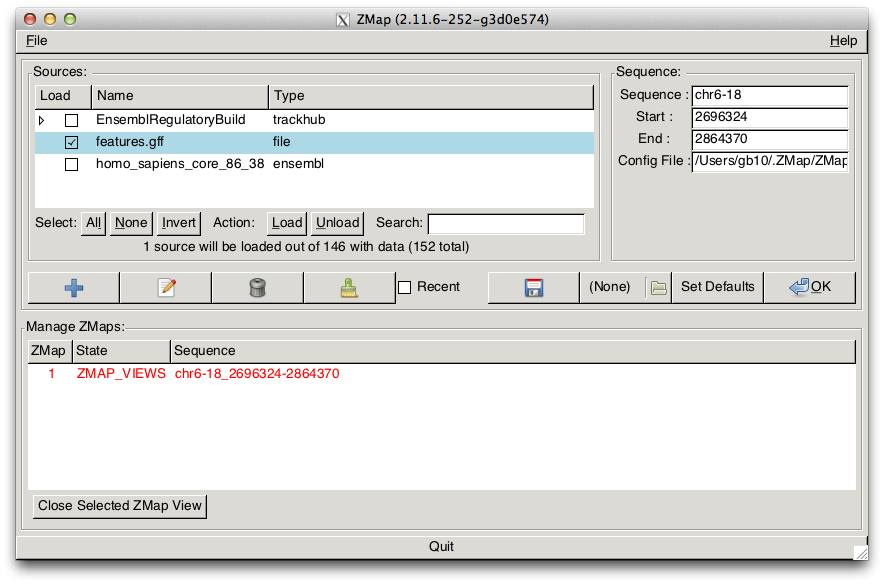
\includegraphics[resolution=150]{images/main_window.png}
\caption{ZMap's Main Window. Use the '+' button to add new sources, enter the sequence details for the region you want to view, and then click 'OK' to start ZMap.}
\label{img_main_window}
\end{figure}

Create one or more sources from which to load data (see section \ref{sec_managing_sources}). Then enter the sequence details for the region you want to load. Click \lstinline{OK} to start a ZMap instance on that region using the selected sources.

You can start a new ZMap with a different region or different sources at any time by editing the sources/sequence in the Main Window and hitting OK. This will not affect any existing running ZMaps.

If you want to load additional data into a running ZMap, you should use the Import dialog instead (see section \ref{sec_import}).

You can save the source details to a config file so that they can easily be re-loaded later. Simply click the \lstinline{Save} button and select a file location. To re-use the config, you can either open the Main Window again and select the file using the file chooser button, or you can run ZMap on the file from the command-line as follows:

\begin{lstlisting}
zmap --conf_file=/path/to/file
\end{lstlisting}

\subsection{Managing sources}
\label{sec_managing_sources}
Both the Main Window and Import dialog show the list of sources available in ZMap. Here, you can view existing sources, create new sources, and select which sources to load.

Click on the \lstinline{+} button to add a new source. This will open the Create Source dialog, where you can create a source of one of the following types:

\begin{enumerate}
\item \lstinline{File/URL}: a local or remote file (see section \ref{sec_file})
\item \lstinline{Ensembl}: an Ensembl database (see section \ref{sec_ensembl})
\item \lstinline{Track hub}: a track hub in the \href{http://trackhubregistry.org/}{Track Hub Registry} (see section \ref{sec_trackhub})
\end{enumerate}

After you have created the new source, it will appear in the sources list. You can enter multiple new sources in the same way. If you want to delete a source, select it in the list and click the delete button, or click the edit button to edit the selected source's details.

Note that for track hub sources, a single hub may contain many data tracks. These are shown as child sources in the list. There will be a small triangle expander icon to the left of the source name to indicate that it contains child sources. There may be an hiercarchy several levels deep depending on the hierarchy of the track hub.

To mark sources for loading, tick the check button in the Load column. Note that selecting a parent source will also select all of its child sources. The text at the bottom of the list will show you how many sources are currently selected for loading, e.g. figure \ref{img_import} shows that ``20 sources will be loaded out of 146 with data (152 total)''. This means that under the selected ``ProjectedSegments'' and ``RegBuildOverview'' sources there are 20 child sources containing data. There are 152 sources in total, but 6 of these are parent sources that just exist to construct the hierarchy and do not contain data themselves, so there are 146 sources in total that contain data.

There are some convenience buttons at the bottom of the sources list to help you find and mark sources, e.g. if you click the \lstinline{All} button and then click the \lstinline{Load} button, all sources will be marked for loading. You can select multiple rows in the sources list using Shift or Ctrl while clicking with the mouse button, and the use the \lstinline{Load} and \lstinline{Unload} buttons to mark/unmark the selected sources for loading.

Typing some text in the \lstinline{Search} box will jump to the first source whose name matches that text. You can jump to the next/previous match with the down/up arrows. Note that the search will only find visible rows, so expand any parent sources first if you also want it to act on child sources.

\subsubsection{File/URL}
\label{sec_file}
To add a new File source, select \lstinline{File/URL} on the Create Source dialog. Click the file chooser button, or type the path/URL of the file into the box. The source name will be taken from the file name by default if you use the file chooser; otherwise you must specify a source name manually. The source name can be anything you like but must be unique and must not contain any special characters (except underscores or dashes). The file can be in any of the file formats supported by ZMap:

\begin{enumerate}
\item GFF3
\item BAM/SAM/CRAM
\item VCF/BCF
\item Bed/bigBed/bigWig
\end{enumerate}

\begin{figure}
\centering
\color[rgb]{0.30980393,0.5058824,0.7411765}
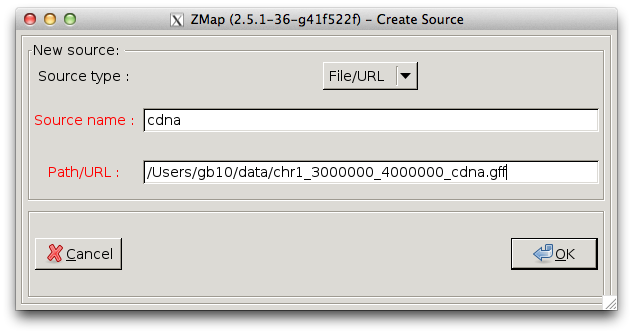
\includegraphics[resolution=150]{images/create_source_file.png}
\caption{Create a new file source}
\label{img_create_source_file}
\end{figure}

\subsubsection{Ensembl}
\label{sec_ensembl}
To create an Ensembl source, select \lstinline{Ensembl} on the Create Source dialog. A host and user/password is required for the source you want to load data from. The public Ensembl host details are pre-filled for you by default. You may change these if you wish but the public host should be fine for most users (note that a password is not required).

\textbf{Selecting a database}
\label{sec_ensembl_select_database}

You need to select which database you wish to load data from. You can type the database name into the \lstinline{Database} box if you know it, or click the search button (the magnifying glass icon) next to the \lstinline{Database} box to search for available databases from the current host. On the search results dialog (figure \ref{img_create_source_ensembl_search_db}), select the database from the list shown and click OK (or double-click to quickly select a database and OK the dialog at the same time).

You can use the Search and Filter boxes to help find a specific database in the list. When you type some text in the Search box, the selection will jump to the first row matching that text. You can press the down array to jump to the next row matching the text. In the Filter dialog, you can type some text and press Enter to filter the list by items containing that text. Click the Clear button to reset back to the original list.

\textbf{Selecting featuresets/biotypes}

On the Create Source dialog, you may optionally enter a list of featuresets and/or biotypes that you want to load. In this case, ZMap will only load features of those types; otherwise, ZMap will load all of the features from the database. Click the search button (magnifying glass icon) next to the Featuresets or Biotypes box to search for available featuresets/biotypes in the current database.

The search results list works in the same way as the database search results dialog, except that you can select multiple featuresets/biotypes by holding down Ctrl (for individual selection) or Shift (for range selection) when you click with the mouse button. When you click OK, this will create a semi-colon separated list on the Create Source dialog. You can also manually type in a semi-colon separated list of featureset/biotype names.

\textbf{Loading DNA}

Tick the \lstinline{Load DNA} button on the Create Source dialog to tell ZMap to load the DNA for the reference sequence from this database. This is not recommended for very large regions because ZMap will need to store all of the sequence for the region in memory, and will also calculate and store the 3-frame translation.

\begin{figure}
\centering
\color[rgb]{0.30980393,0.5058824,0.7411765}
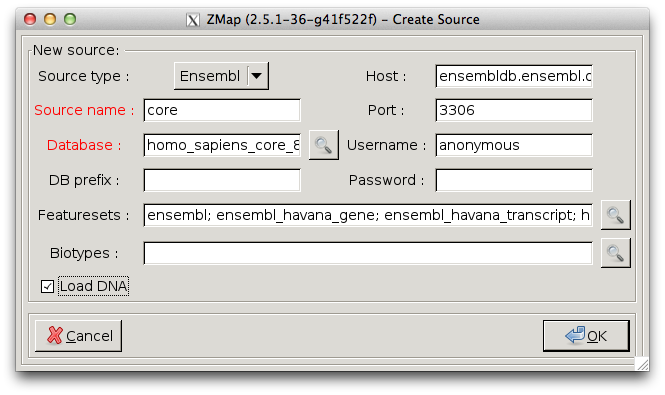
\includegraphics[resolution=150]{images/create_source_ensembl.png}
\caption{Create a new Ensembl source. Click on the magnifying glass icons to search for databases/featuresets/biotypes to load.}
\label{img_create_source_ensembl}
\end{figure}

\begin{figure}
\centering
\color[rgb]{0.30980393,0.5058824,0.7411765}
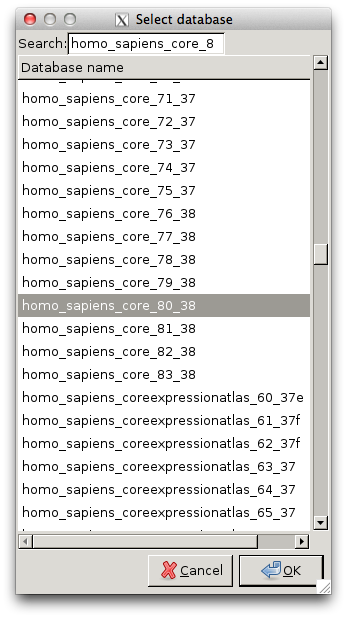
\includegraphics[resolution=150]{images/create_source_ensembl_search_db.png}
\caption{Search a list of available Ensembl databases. Type text in the Search box to jump to items containing that text. You can use the up/down arrows to jump to the next/previous item with the same text.}
\label{img_create_source_ensembl_search_db}
\end{figure}

\subsubsection{Track  hub}
\label{sec_trackhub}
ZMap can load data from a collection of tracks in a track hub using the \href{http://trackhubregistry.org/}{Track Hub Registry}. You can search for existing track hubs or register and manage new ones.

\textbf{Searching for track hubs}

To search for track hubs in the registry, press the Search button on the Create Source dialog. This will open the Search dialog (figure \ref{img_create_source_trackhub_search}). In the \lstinline{Search text} box you can enter any query to search for. The search is case insensitive and you can use wildcards, regular expressions and powerful, advanced search operations such as proximity searches. See the documentation here for details: \url{http://trackhubregistry.org/docs/search}. 

You may also filter the results by specifying the species, assembly or hub. These fields are case sensitive and must be entered exactly as they appear in the registry, e.g. ``Mus musculus'' and not ``Mus Musculus''. If you are not sure of the case, it is generally fine to use the \lstinline{Search text} box instead, e.g. at the time of writing, searching for ``mus musculus'' in the \lstinline{Search text} box gives the same results as searching for ``Mus musculus'' in the species box, while searching for ``mouse'' returns one extra, spurious match from a different species which happens to contain the text ``mouse'' somewhere in its description.

After clicking OK on the search dialog, you will be presented with a list of results. You can search/filter the results list in the same manner as the Ensembl search results dialog (see section \ref{sec_ensembl_select_database} and figure \ref{img_create_source_ensembl_search_db}).

\begin{figure}
\centering
\color[rgb]{0.30980393,0.5058824,0.7411765}
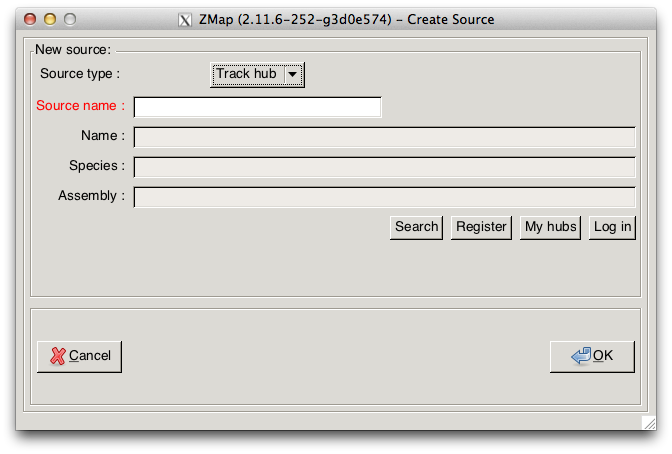
\includegraphics[resolution=150]{images/create_source_trackhub.png}
\caption{Create a new Track Hub source. Click on the Search button to search the Track Hub Registry, or Register to register a new one. Click My Hubs to view all of the track hubs you have registered.}
\label{img_create_source_trackhub}
\end{figure}

\begin{figure}
\centering
\color[rgb]{0.30980393,0.5058824,0.7411765}
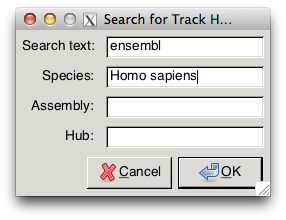
\includegraphics[resolution=150]{images/create_source_trackhub_search.png}
\caption{Search for hubs in the Track Hub Registry. The Search Text is case insensitive and can contain wildcards. The other fields are case sensitive and must be entered exactly.}
\label{img_create_source_trackhub_search}
\end{figure}

\textbf{Register a track hub}

ZMap provides the facility to register and manage track hubs in the Track Hub Registry. For this you will first need to sign up for an account on \url{http://trackhubregistry.org/}. To register a new track hub, click the Register button on the Create Source dialog. You will be prompted to log in (if you have not already logged in during the current ZMap session). You will then be asked to enter details about the new track hub (figure \ref{img_create_source_trackhub_register}).

The only mandatory field is the URL. This is the url of the main track hub file, which is usually named hub.txt, e.g. \url{http://genome-test.cse.ucsc.edu/~hiram/hubs/Plants/hub.txt}.

The Assemblies field is only required if the hub genome subdirectory names are not valid UCSC DB names. In this case you must provide a map from the hub's genome names to their corresponding INSDC accessions as a semi-colon separated list of key=value pairs, e.g.
\begin{lstlisting}
araTha1=GCA_000001735.1 ; ricCom1=GCA_000151685.2
\end{lstlisting}

You can use the Type field to enter the type of the assembly data contained in the hub, which can be one of "genomics", "epigenomics", "transcriptomics", "proteomics" (default: "genomics"). By specifying the type you allow the user to search for track hubs based on particular types.

\begin{figure}
\centering
\color[rgb]{0.30980393,0.5058824,0.7411765}
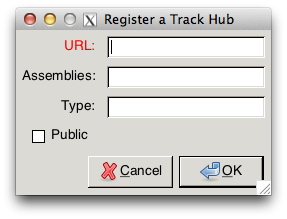
\includegraphics[resolution=150]{images/create_source_trackhub_register.png}
\caption{Register a hub in the Track Hub Registry. Enter the URL of the hub.txt file and optionally a mapping of genome names to UCSC DB names and the type. Tick the Public box if you want the track hub to be publically searchable.}
\label{img_create_source_trackhub_register}
\end{figure}

\textbf{Managing registered track hubs}

You can use the My Hubs button on the Create Source dialog to view a list of all track hubs that you have registered via your account. You will be asked to log in if necessary before you can view your hubs. This will open a dialog showing a list of all the hubs you have registered (figure \ref{img_create_source_trackhub_view}). The list shows each genome in the hub on a separate line. Select one of the hubs in the list and click OK to use it as a source.

\begin{figure}
\centering
\color[rgb]{0.30980393,0.5058824,0.7411765}
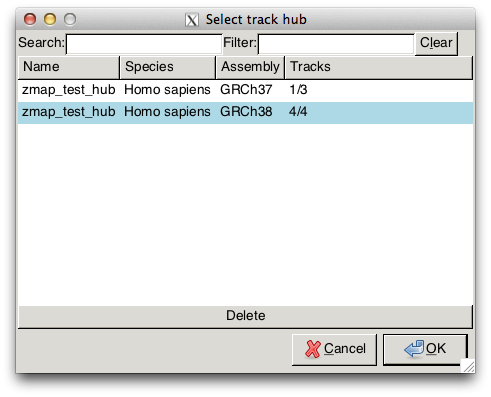
\includegraphics[resolution=150]{images/create_source_trackhub_view.png}
\caption{View any hubs you have registered in the Track Hub Registry.}
\label{img_create_source_trackhub_view}
\end{figure}

You can also use this dialog to delete your track hubs from the registry. Select a hub from the list and press the Delete button, and then click OK on the confirmation dialog. Note that this will only delete the selected genome from the registry, so to delete all of the genomes for a hub you will need to select and delete them separately. Note that deleting a hub only deletes it from the Track Hub Registry; it does not affect the original data at all.

Track hubs can also be managed directly via your dashboard at \url{http://trackhubregistry.org/}.

\textbf{Logging in/out}

You will be prompted to log if necessary any time you attempt to register a hub or view registered hubs. You can also use the \lstinline{Log in} button on the Create Source dialog. If you want to log in with a different account, you can first log out using the \lstinline{Log out} button on the Create Source dialog.


\subsection{Running ZMap with a config file}
If you have several sources, it can be convenient to specify them in a config file rather than typing them on the command-line. You can also then set up many different options and styles to use for these sources. The following config file shows examples of a GFF file source, an ensembl source and a track hub source. The ensembl and track hub sources are delayed but the GFF file source will be loaded on startup.

\begin{lstlisting}
#
# The ZMap stanza contains general ZMap properties
#

[ZMap]
# The list of sources
sources=features ; homo_sapiens_core_86_38 ; EnsemblRegulatoryBuild

# Sequence name/start/end can be specified here, on the command-line, or
# omitted if they are to be taken from the file
sequence=chr6-18
start=2696324
end=2864370

# Custom styles file to control the display properties of features
stylesfile=/Users/gb10/work/checkout/annotools/zmap/examples/styles.ini

#
# Source stanzas (one per source)
#

[features.gff]
url=file:////Users/gb10/work/checkout/annotools/zmap/examples/features.gff

[homo_sapiens_core_86_38]
url=ensembl://anonymous:@ensembldb.ensembl.org:3306?db_name=homo_sapiens_core_86_38
featuresets=ensembl; ensembl_havana_gene; ensembl_havana_transcript; havana
delayed=true

[EnsemblRegulatoryBuild]
url=trackhub:///AVgdMa38PO47wJF0u-tI
delayed=true
\end{lstlisting}

ZMap can be started by passing the config file on the command line:
\begin{lstlisting}
zmap --conf_file=/path/to/file
\end{lstlisting}

Alternatively, the config file can be saved as \lstinline{~/.ZMap/ZMap} and will be picked up by default (although it is recommended not to include the sequence details in this case because it can cause confusion).

\subsection{Starting ZMap from Otter}
ZMap is opened via the Tools menu bar in Otter (figure \ref{img_open_from_otterlace}).

\begin{figure}
\centering
\color[rgb]{0.30980393,0.5058824,0.7411765}
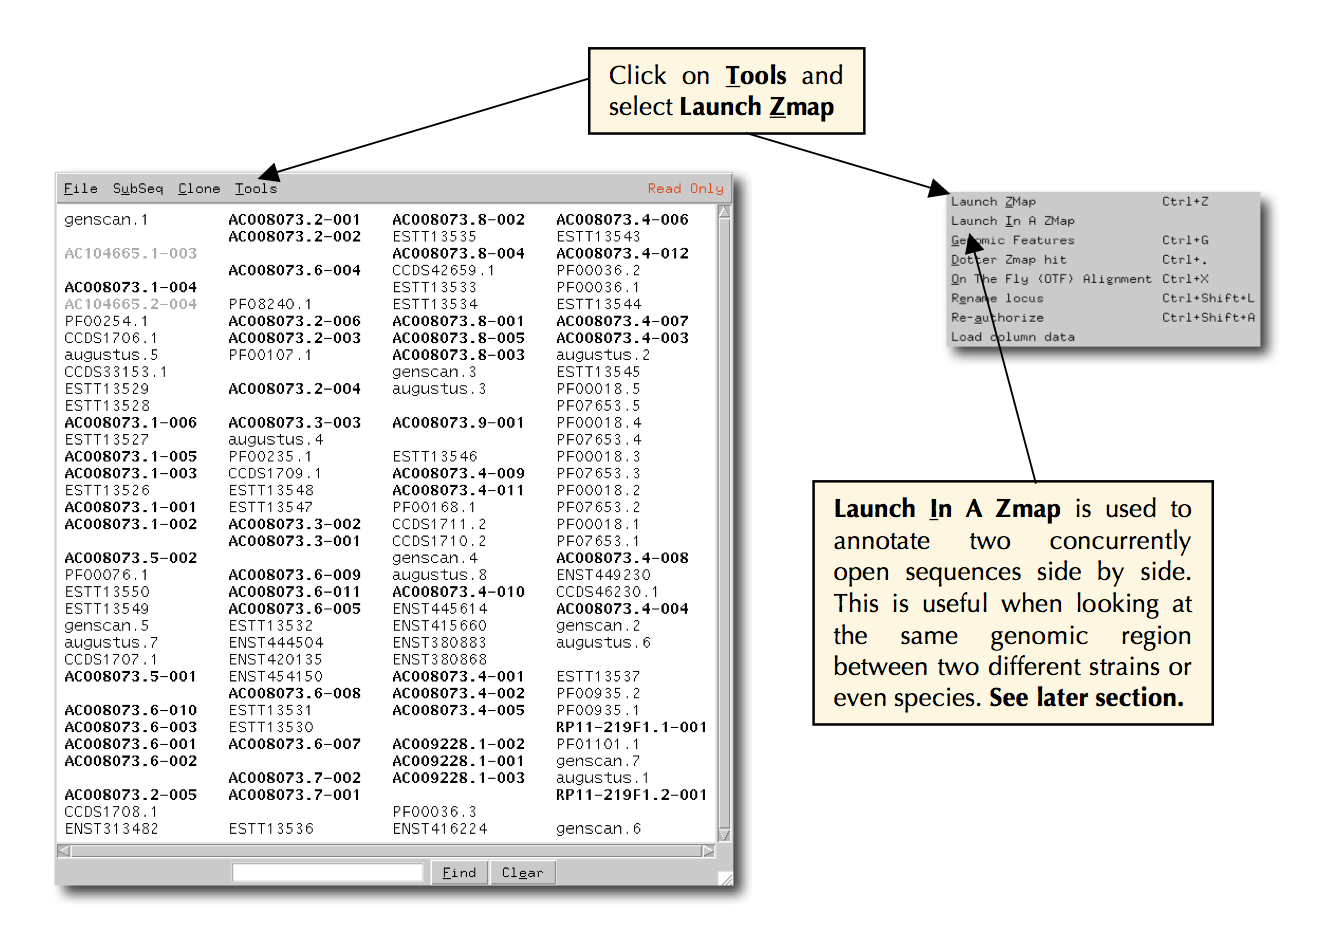
\includegraphics[width=15.231cm]{images/open_from_otterlace.png}
\caption{Opening ZMap from Otter}
\label{img_open_from_otterlace}
\end{figure}

\subsection{Importing data into an existing ZMap}
\label{sec_import}
You do not need to load all data up front when you first start ZMap. Data from all types of source can be loaded on the fly into an existing ZMap instance using the Import dialog. Data can be loaded for the entire region in the ZMap instance, or just a sub-region.

Optionally, you can first set the mark if you want to load data just into a specific marked region.

To open the Import dialog (figure \ref{img_import}), go to the \lstinline{File} menu and select \lstinline{Import}, or press \lstinline{Ctrl-I}.

At the top of the Import dialog is a section showing the sequence region that you are importing data into. If the mark is set, then the default range will be taken from the mark; otherwise it will be the full ZMap range. You can edit the values to whatever you want.

Note that the sequence name is the name the ZMap will attempt to look up in the source. This may be different to the sequence name in ZMap and must be edited to be a valid name in the source. If you are loading data from sources with different name formats then you must load them separately (chromosome names in Ensembl are generally just the digit, e.g. ``1'', while in track hubs they tend to be prefixed with ``chr'', e.g. ``chr1''). If you get the name wrong, ZMap will pop up a warning telling you what sequence names are available in the source when you attempt to load the data.

The greyed-out sequence details on the bottom right of the dialog show the original sequence name and full range in ZMap. This is just for reference.

\begin{figure}
\centering
\color[rgb]{0.30980393,0.5058824,0.7411765}
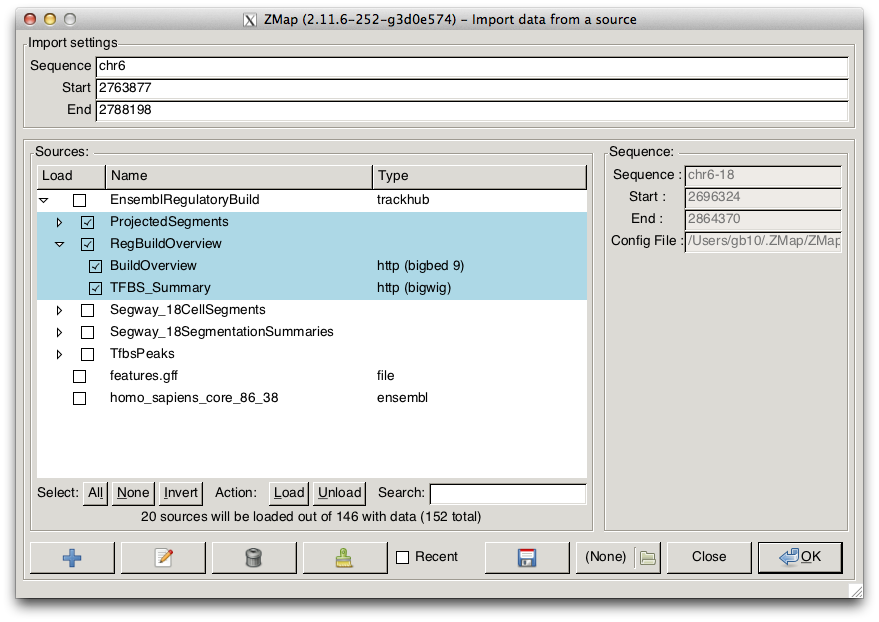
\includegraphics[width=15.231cm]{images/import.png}
\caption{The Import dialog}
\label{img_import}
\end{figure}

When you have specified the region, you must then select some source(s) to load data from (see section \ref{sec_managing_sources}). By default, only recent sources are shown (that is, sources you have added manually via the Import dialog), so the sources list will be empty when you first open the Import dialog. If you want to see all sources, untick the \lstinline{Recent} button. If you want to clear the list of recent sources, click the clear button - this will clear the list of sources that are shown when \lstinline{Recent} is ticked, but all sources will still be available when \lstinline{Recent} is unticked.

When you have selected all of the sources you want to load, click OK, and ZMap will start loading the data.


\clearpage
\section{The ZMap interface}

The main ZMap display (figure \ref{img_main_interface}) consists of a canvas, which is a drawing area where any analysis and annotation that is present in your region of interest is shown. There is a toolbar, information bar and menu at the top, and a ruler showing the coordinates at the current position based on the current coordinate system. There is also a navigator pane to the left of the ruler, which is hidden by default.

\begin{figure}
\centering
\color[rgb]{0.30980393,0.5058824,0.7411765}
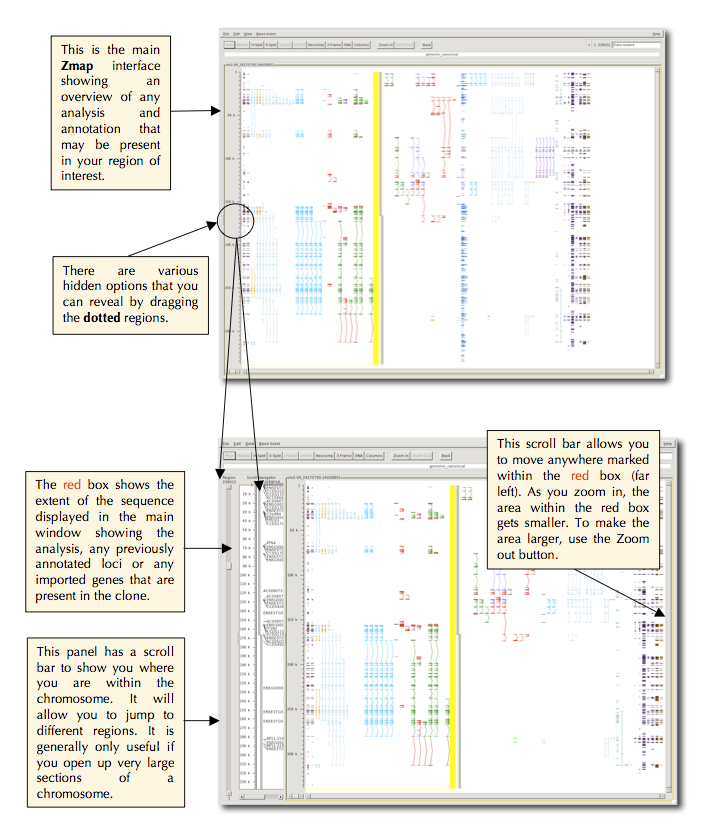
\includegraphics[width=15.231cm]{images/main_interface.png}
\caption{The main ZMap interface}
\label{img_main_interface}
\end{figure}


\subsection{Navigating around the canvas}
Navigate by using the scroll bars or the middle mouse button (figure \ref{img_navigating}). By clicking the middle mouse anywhere in ZMap you will see a horizontal line. You can move this up and down and the coordinate of the clicked position will be displayed along the line. By default the coordinate display is relative to the start of the loaded region. To toggle to toplevel coordinates, go to the main menu and select \lstinline{View -> Toggle coords}.

When the button is released, the window will refresh, centering on the position of the line. You can also click in the window to make it active and use the scroll wheel to navigate up and down or achieve the same result using the scroll bar on the right hand side of the window.

If you release the mouse outside the ZMap window, you can then check the sequence position displayed, without re-centering.

\begin{figure}
\centering
\color[rgb]{0.30980393,0.5058824,0.7411765}
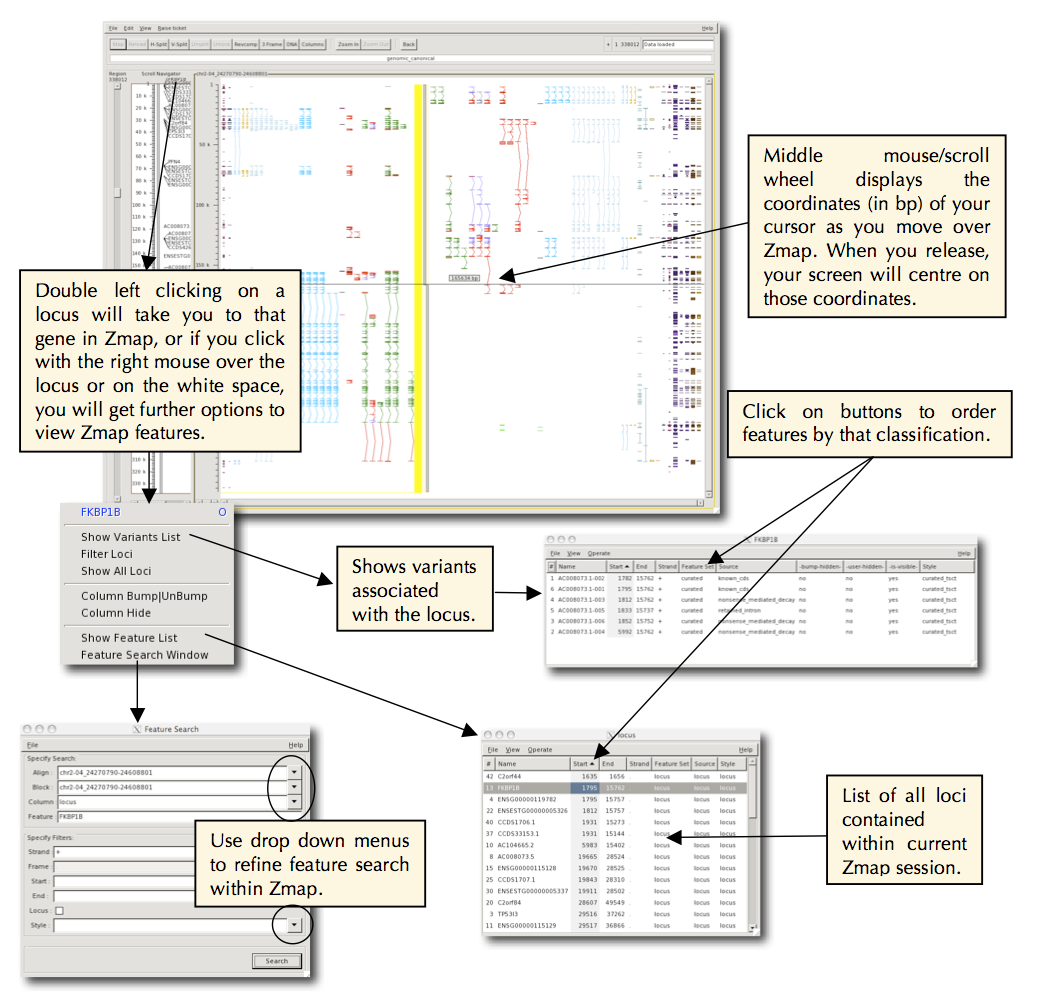
\includegraphics[width=15.231cm]{images/navigating.png}
\caption{Navigating}
\label{img_navigating}
\end{figure}


\subsection{Zooming} \label{sec_zooming}
See figure \ref{img_zooming}.

\begin{itemize}
\item Zoom in by using the \lstinline{Zoom in}/\lstinline{Zoom out} buttons on the toolbar
\item Right-click on the toolbar buttons for more options, e.g. to zoom all the way in or out
\item Draw with the left mouse button to lasso an area to zoom in to
\item Press the \lstinline{z} key on the keyboard to zoom to the current focus feature.
\item Use the \lstinline{Z} key to zoom to a whole transcript if you have one or more exons highlighted, or all HSPs if you have one HSP highlighted (HSPs are the ``blocks'' that you see in the homology columns, such as ESTs and protein hits). 
\end{itemize}

\begin{figure}
\centering
\color[rgb]{0.30980393,0.5058824,0.7411765}
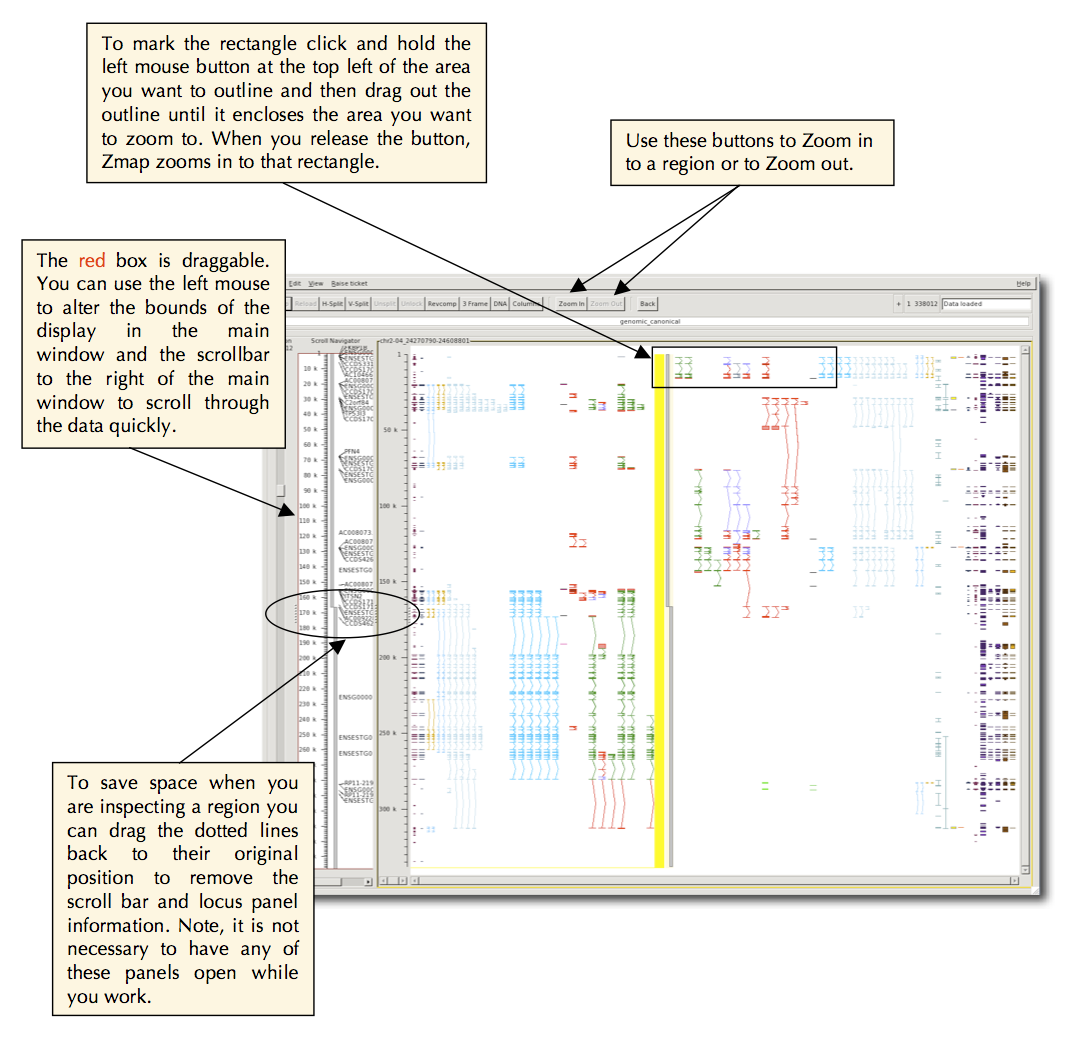
\includegraphics[width=15.231cm]{images/zooming.png}
\caption{Zooming}
\label{img_zooming}
\end{figure}


\subsection{Toolbar} \label{sec_toolbar}
Many functions are available from the toolbar section in ZMap. Below the toolbar is an information bar, which displays information about the current focus feature. See figures \ref{img_toolbar_feature_details} and \ref{img_feature_display_details}.

\begin{itemize}
\item \textbf{Stop} - Stop loading of data and reset ZMap
\item \textbf{Reload} - Reload data after a reset
\item \textbf{Back} - Return to the previous location / zoom level
\item \textbf{H-Split} - Split the window horizontally (see section \ref{sec_split})
\item \textbf{V-Split} - Split the window vertically (see section \ref{sec_split})
\item \textbf{Unsplit} - Remove the currently-active split pane (click in a pane first to make it active)
\item \textbf{Revcomp} - Reverse complement the sequence view
\item \textbf{3-Frame} - Show the 3-frame translation. Right-click on this button to show more options (see \ref{sec_dna_3_frame})
\item \textbf{DNA} - Show the reference sequence DNA  (see \ref{sec_dna_3_frame})
\item \textbf{Columns} - Open the Track Configuration dialog (see section \ref{sec_track_configuration})
\item \textbf{Zoom In} - Zoom the display in by x2 (right-click for more options - see section \ref{sec_zooming})
\item \textbf{Zoom Out} - Zoom the display out by x2 (right-click for more options - see section \ref{sec_zooming})
\item \textbf{Filter} - This spinwheel box allows you to set a score cutoff for features in the active column (see section \ref{sec_filter})
\item \textbf{Current strand} - Shows as ``+'' for the forward strand or ``-'' for the reverse strand
\item \textbf{Current range} - Shows the extent of the current range
\item \textbf{Loading status} - Shows the status of columns during loading
\end{itemize}

\begin{figure}
\centering
\color[rgb]{0.30980393,0.5058824,0.7411765}
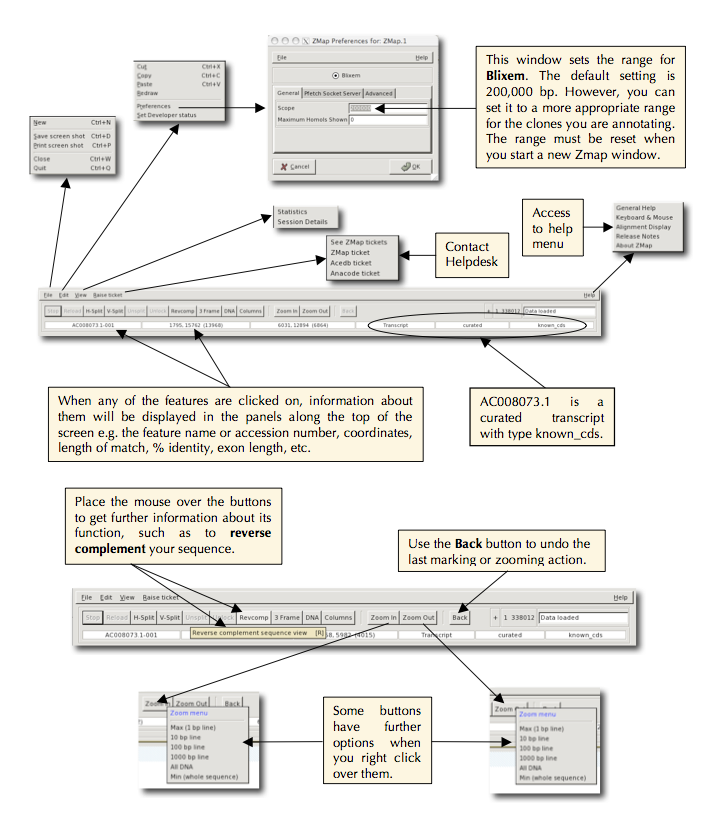
\includegraphics[width=15.231cm]{images/toolbar_feature_details.png}
\caption{Toolbar feature details}
\label{img_toolbar_feature_details}
\end{figure}

\begin{figure}
\centering
\color[rgb]{0.30980393,0.5058824,0.7411765}
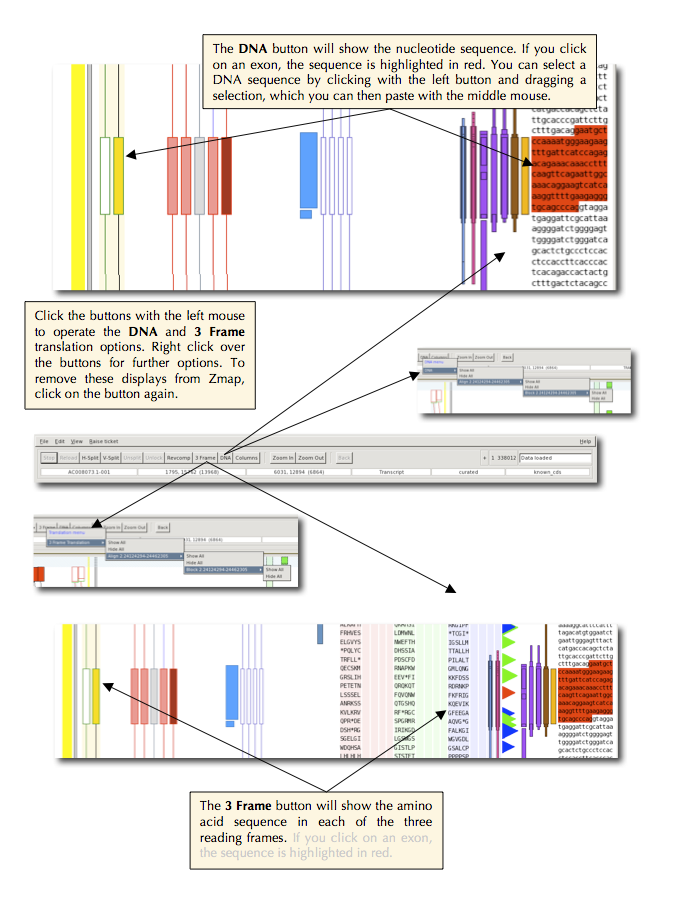
\includegraphics[width=15.231cm]{images/feature_display_details.png}
\caption{Feature display details}
\label{img_feature_display_details}
\end{figure}


\subsection{Menu bar}
\subsubsection{File menu}
\begin{itemize}
\item \textbf{New Sequence} - Create a new view in the current ZMap session (see section \ref{sec_multiple_views})
\item \textbf{New Source} - Create and load a new source into the existing region
\item \textbf{Save} - Save all of the features to a GFF file (without prompting if a file has previously been selected)
\item \textbf{Save As} - Save all of the features to a GFF file (prompting for a new file name)
\item \textbf{Import} - Import features from a local or remote file (e.g. BAM/GFF)
\item \textbf{Export} - Export features, config, styles or reference sequence DNA
\item \textbf{Save screen shot} - Save the current canvas as a screen shot
\item \textbf{Print screen shot} - Open the print dialog to print the current canvas
\item \textbf{Close} - Close the current ZMap window
\item \textbf{Quit} - Disconnect from all servers and quit ZMap
\end{itemize}

\subsubsection{Edit menu}
\begin{itemize}
\item \textbf{Copy Feature Coords} - Copy the currently-selected feature coordinates to the clipboard in the format: \lstinline{<seqname>:<start>-<end>}
\item \textbf{Copy Feature Coords (CHR)} - As above but prefix the seqname with \lstinline{chr}
\item \textbf{Paste Feature Coords} - Get feature coordinates in the above format from the clipboard and zoom the ZMap display to that region
\item \textbf{Redraw} - Redraw the canvas
\item \textbf{Styles} - Show the Styles dialog (see section \ref{sec_style_configuration})
\item \textbf{Preferences} - Open the Preferences dialog (see section \ref{sec_preferences})
\end{itemize}

\subsubsection{View menu}
\begin{itemize}
\item \textbf{Session details} - View details about the current ZMap session (useful when reporting bugs)
\item \textbf{Toggle coords} - Toggle between 1-based and toplevel coordinate systems (see \ref{sec_ruler})
\end{itemize}

\subsubsection{Raise Ticket menu}
Use this menu to raise a ticket to report a bug or request a new feature.

\subsubsection{Help menu}
The help menu contains links to various quick-access help pages, as well as a link to the release notes (to find out what's new in the latest version). The \lstinline{About ZMap} menu item will tell you exactly which version of ZMap you are running.


\subsection{Coordinate display (ruler)} \label{sec_ruler}
The ruler to the left of the canvas shows the coordinates in the current coordinate system. By default, ZMap uses a local coordinate system, which starts at 1 for the first coordinate in the loaded region. You can toggle to the real toplevel coordinates using the menu option \lstinline{View->Toggle coords}.


\subsection{Navigator pane}
The navigator pane is on the left of the ZMap display but is hidden by default. It can be exposed by dragging the drag bar to the left of the ruler.

The navigator pane shows the analysis, any previously annotated loci or any imported genes that are present in the clone. Double-clicking on a locus will take you to that gene in ZMap. Right-click to show various other options.

The extent of the current canvas is shown by a red outline in the navigator. This is the region that can be scrolled using the scrollbars in the main canvas area. Zooming in or out on the main canvas changes the size of this box. Alternatively you can drag the red box to scroll the current canvas area, or drag the bounds of the red box to change the zoom level of the main canvas area. See figures \ref{img_main_interface} and \ref{img_navigating}.


\subsection{Splitting the window} \label{sec_split}
Use the \textbf{split window} functionality to effectively reduce the size of the window when looking at homologies. This is of particular use when you have to deal with very large introns because you can essentially reduce the introns to whatever size you wish, or when there are very many HSPs, because you can keep your gene object in view and static, but still scroll across the evidence. See figure \ref{img_split_window}. You may split the window both horizontally and/or vertically as many times as you wish.

By default, the windows will be locked and will scroll in unison. You can unlock them by pressing the \lstinline{Unlock button} and they will then scroll independently.

\begin{figure}
\centering
\color[rgb]{0.30980393,0.5058824,0.7411765}
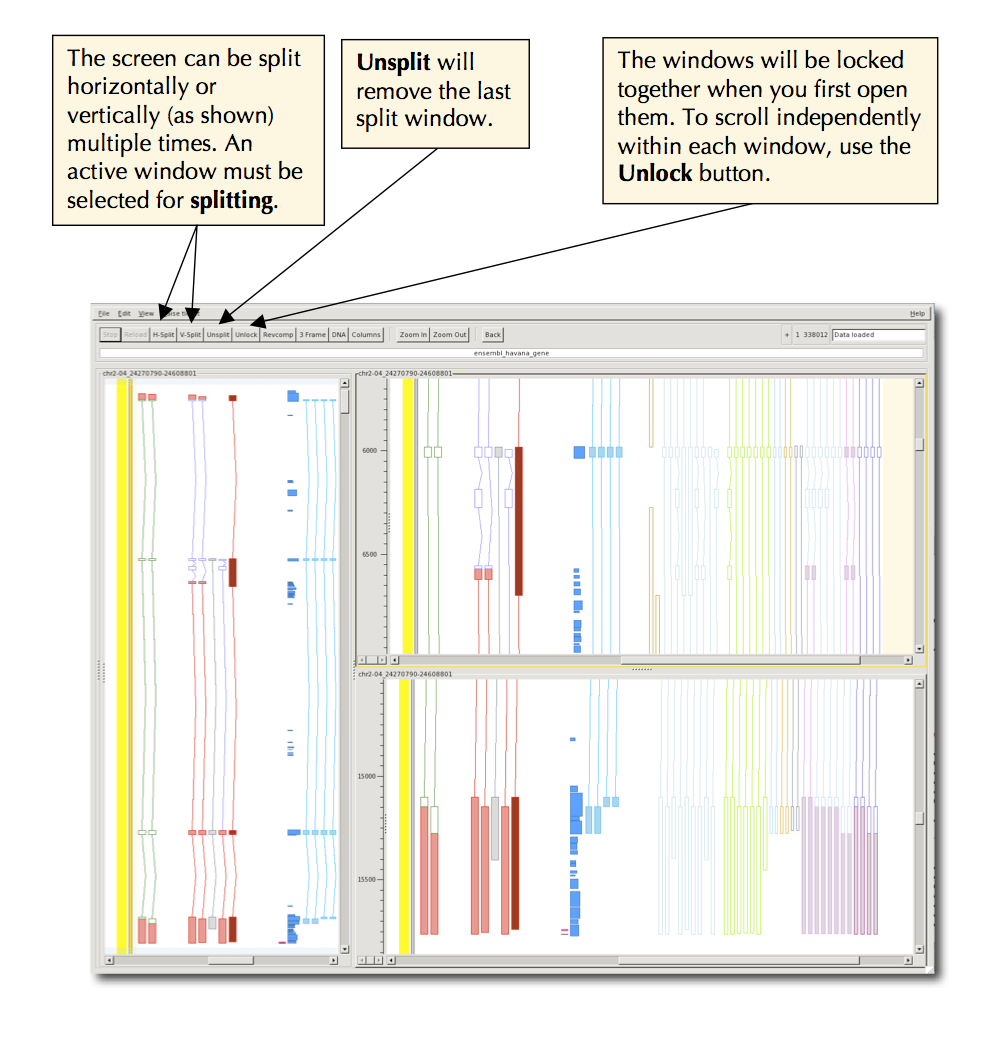
\includegraphics[width=15.231cm]{images/split_window.png}
\caption{Splitting windows}
\label{img_split_window}
\end{figure}


\subsection{DNA and 3-frame translation} \label{sec_dna_3_frame}
You can show the reference sequence DNA and/or 3-frame translation by pressing the \lstinline{DNA} and \lstinline{3-Frame} buttons on the toolbar respectively. Click the buttons again to turn them off.

Right-click on the \lstinline{3-Frame} buttons for these additional options:
\begin{itemize}
\item \textbf{None} - Turn all 3-frame columns off
\item \textbf{Features} - Show ``3-frame sensitive'' features split into separate columns for each reading frame
\item \textbf{3 Frame Translation} - Show the 3-frame translation (default)
\item \textbf{Features + 3 Frame Translation} - Show 3-frame sensitive features alongside the 3-frame translation
\end{itemize}

When you select a gene object, the exons will be highlighted in the DNA and 3 Frame columns in the following colours (see figure \ref{img_dna_3_frame}):
\begin{itemize}
\item \textbf{Red} - UTR
\item \textbf{Light green} - CDS
\item \textbf{Dark green} - CDS (indicates the current frame in the 3-frame display)
\item \textbf{Yellow} - Split codon (start)
\item \textbf{Orange} - Split codon (end) 
\end{itemize}

\begin{figure}
\centering
\color[rgb]{0.30980393,0.5058824,0.7411765}
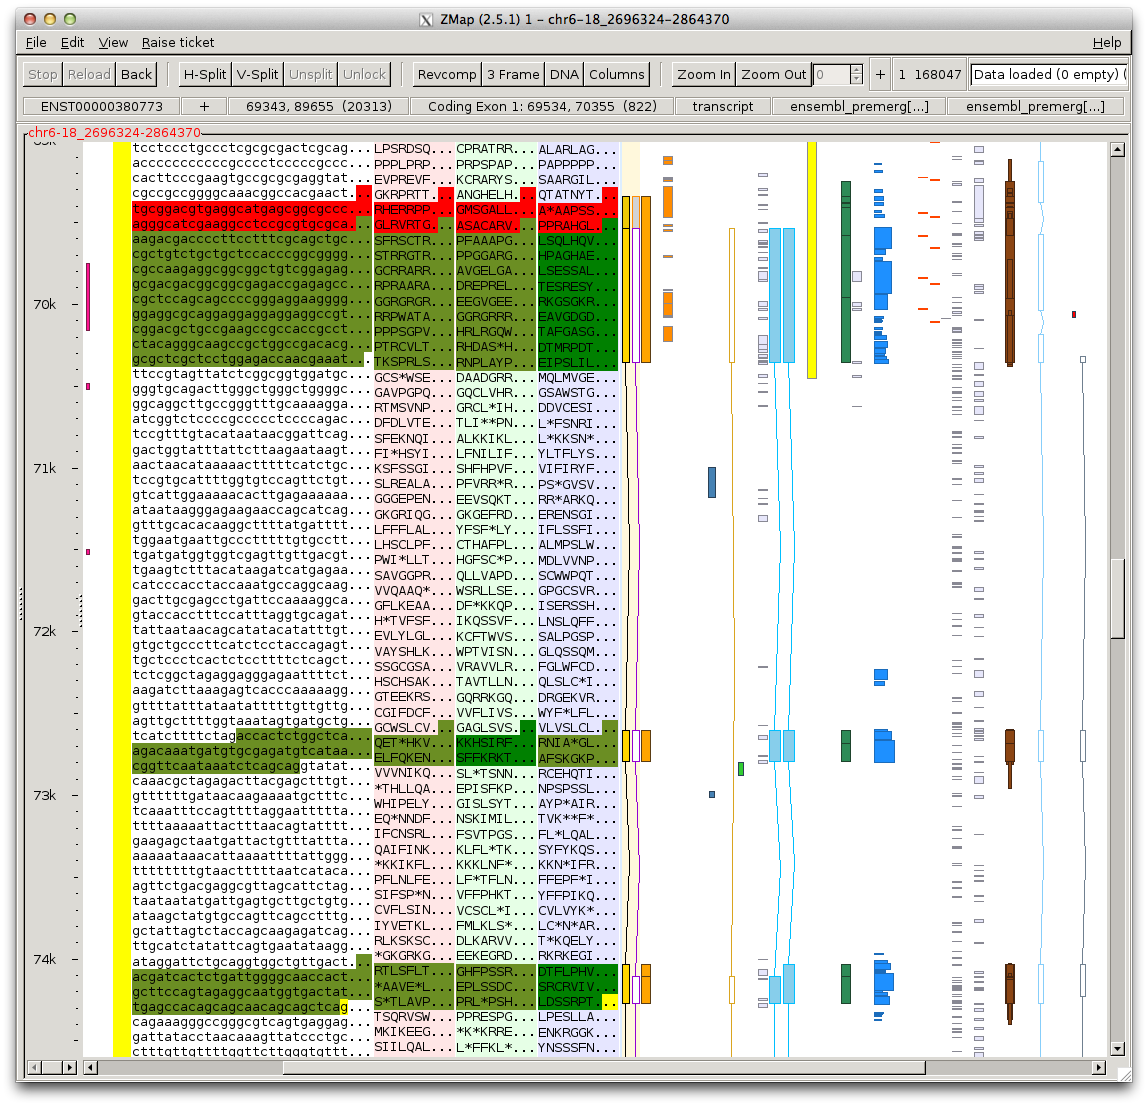
\includegraphics[width=15.231cm]{images/dna_3_frame.png}
\caption{DNA and 3-frame translation in ZMap. When a gene object is selected, the sequence is highlighted red for UTR and green for CDS. The darker green indicates the current frame}
\label{img_dna_3_frame}
\end{figure}


\clearpage
\section{Feature selection}

\subsection{The Focus Feature}
If you click on a column background then that column becomes the ``focus'' column and you can do various short cut operations on it such as pressing \lstinline{b} to bump it. If you click on a feature then that feature becomes the ``focus'' feature and similarly you can do various short cut operations on it such as zooming in to it. (Note when you select a feature then its column automatically becomes the focus column.)


\subsection{Selecting multiple features}
\begin{itemize}
\item If you left click once on a feature in ZMap, you will highlight all of its exons, the coordinates of which are now stored in the paste buffer and can be copied elsewhere, such as into the transcript editing window in Otter.
\item You can select multiple features by holding the Shift key down and left clicking with mouse (same as for multi select on the Mac, Windows etc). This option will highlight a single exon at a time for each feature, but the accession numbers of each feature and the individual exon coordinates are held in the paste buffer. This is a particularly useful way of selecting ZMap hits to use in the OTF alignment tool in Otter, as all selected homologies will be held in the paste buffer and automatically pasted into the OTF accession window. Each of the exon coordinates can also be pasted into the transcript editing window in Otter (see figure \ref{img_paste_features}).
\end{itemize}

\begin{figure}
\centering
\color[rgb]{0.30980393,0.5058824,0.7411765}
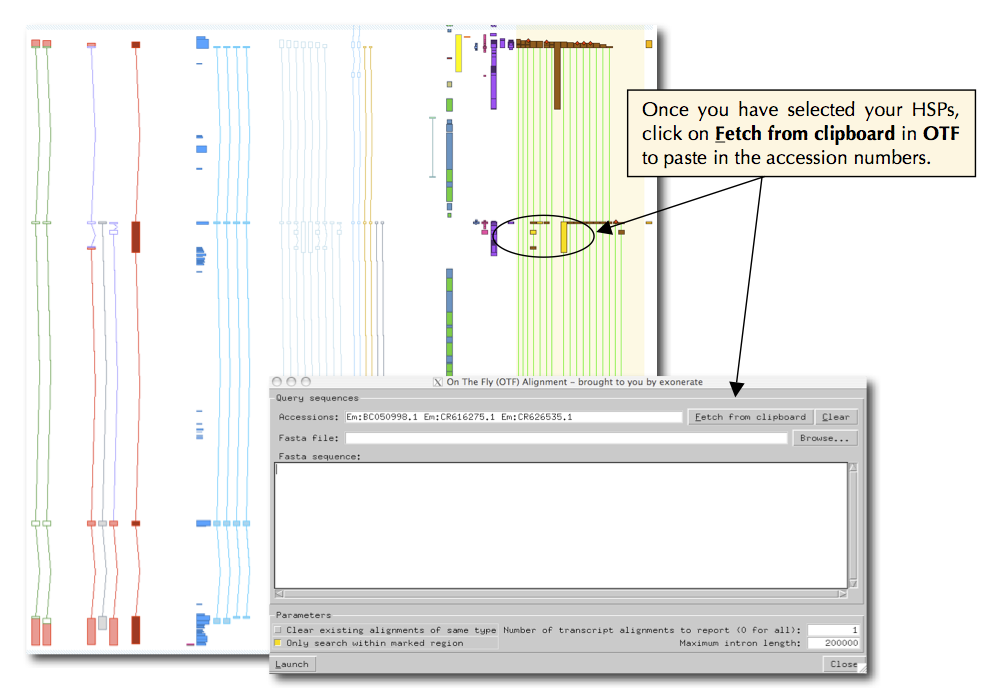
\includegraphics[width=15.231cm]{images/show_hide.png}
\caption{Pasting selected features to Otter's OTF dialog}
\label{img_paste_features}
\end{figure}


\subsection{Hiding features}
You can remove selected features in ZMap by pressing \lstinline{Delete} on the keyboard and restore them by pressing \lstinline{Shift-Delete} (note on the Mac you need to press \lstinline{Fn-Delete} and \lstinline{Shift-Fn-Delete}). This is a particularly useful way of removing evidence that you have already assigned to a transcript object.


\subsection{Marking a region} \label{section_marking_a_region}
While the focus-feature facility is useful, the focus changes every time you click on a new feature. Sometimes you want to select a ``working'' feature or area more permanently. To do this you can ``mark'' a feature or region and it will stay marked until you unmark it (see section \ref{section_marking_a_region}).
 
The ``marked'' area remains clear, while the unmarked area above and below is shaded out with a blue hashed overlay (see figure \ref{img_focus_and_mark}). Working on a marked region is recommended when you have a large amount of data loaded, because operations are faster and the display is less cluttered.

\begin{figure}
\centering
\color[rgb]{0.30980393,0.5058824,0.7411765}
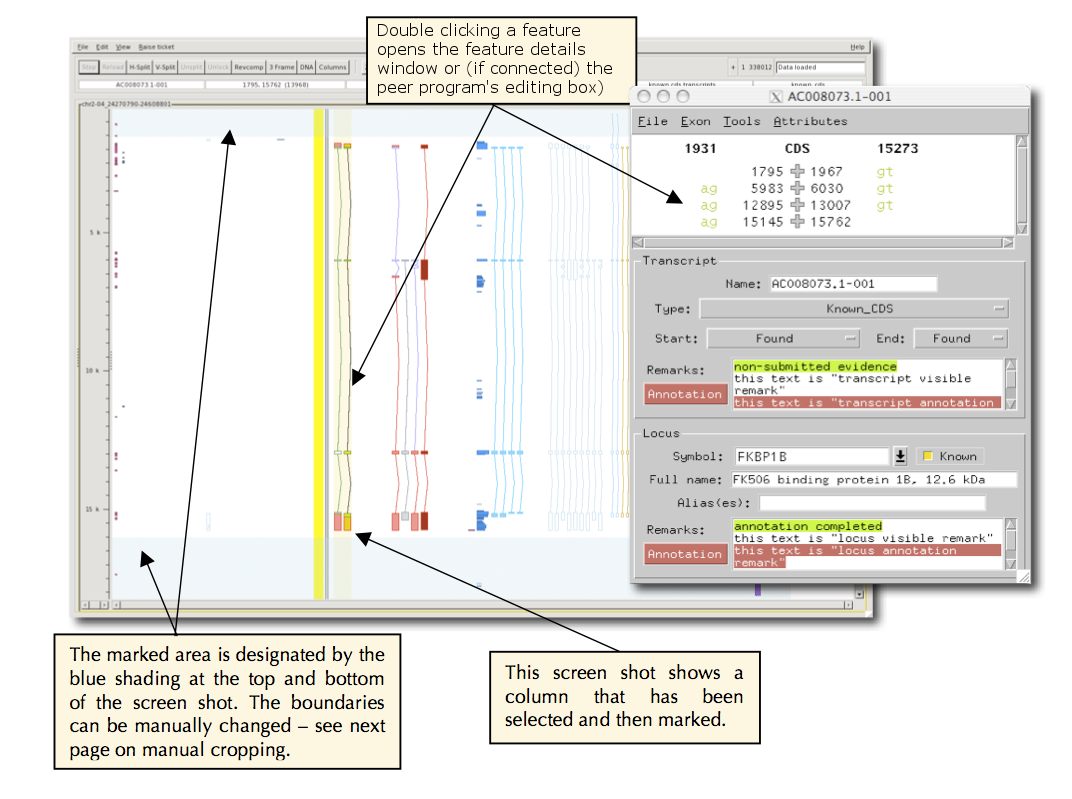
\includegraphics[width=15.231cm]{images/focus_and_mark.png}
\caption{Focus and Mark}
\label{img_focus_and_mark}
\end{figure}

\subsubsection{Mark a feature}
\begin{enumerate}
\item Select a feature to make it the focus feature.
\item Press \lstinline{m} to mark the feature, the feature will be highlighted with a blue overlay.
\end{enumerate}

Feature marking behaves differently according to the type of feature you highlighted prior to marking and according to whether you press \lstinline{m} or \lstinline{M} to do the marking:

\begin{enumerate}
\item  If you press \lstinline{m}, the mark is made around all features you have highlighted, e.g. a whole transcript, a single exon, several HSPs.
\item  If you press \lstinline{M} to do the marking around transcripts the whole transcript becomes the marked feature and the marked area extends from the start to the end of the transcript.
\item  If you press \lstinline{M} to do the marking around alignments all the HSPs for that alignment become the marked feature and the marked area extends from the start to the end of all the HSPs.
\item  If you press \lstinline{M} to do the marking around all other features: the feature becomes the marked feature and the marked area extends from the start to the end of the feature.
\item  If no feature is selected but an area was selected using the left button rubberband then that area is marked.
\item  If no feature or area is selected then the visible screen area minus a small top/bottom margin is marked.
\end{enumerate}

\subsubsection{Mark an area}
\begin{enumerate}
\item Select an area by holding down the left mouse button and dragging out a box to focus on that area.
\item Press \lstinline{m} to mark the area.
\end{enumerate}

\subsubsection{Manual cropping of the marked borders}
You can manually change the borders of the marked area by putting your cursor over this area and using the cropping tool by clicking and holding with the left mouse button and dragging to make the area bigger or smaller.

\subsubsection{Unmark a feature}
Press \lstinline{m} or \lstinline{M} again, i.e. the mark key toggles marking on and off.


\clearpage
\section{Track display options}

\subsection{Bumping tracks}
This section describes how to select a feature, mark it and then zoom in to it and examine evidence that overlaps that feature. The default setting for ZMap is to show HSPs drawn on top of each other. This saves space on the canvas making it easier to see the general features of the region of interest. The bump option allows you to see the HSPs as multiple alignments.
\begin{enumerate}
\item Click on the feature you are interested in (perhaps a transcript)
\item Mark it by pressing \lstinline{m}
\item Zoom in to the feature by pressing either \lstinline{z} or \lstinline{Z} (as described previously).
\end{enumerate}

Now when you bump an evidence column to look at matches that overlap the feature you will find that bumping is much faster because only those matches that overlap the feature get bumped and you also have fewer matches to look at. The quickest way to bump a column is:
\begin{enumerate}
\item Click on the column to select it.
\item Bump it by pressing \lstinline{b} (if you press \lstinline{b} again the column will be unbumped). If you have marked a feature then bumping is restricted to matches that overlap that feature, otherwise bumping is for the whole column.
\end{enumerate}

If you use the default bumping mode (i.e. you pressed \lstinline{b}) then you will find all matches from the same piece of evidence are joined by coloured bars, the colours indicate the level of colinearity between the matches (see figure \ref{img_bumping}).
\begin{enumerate}
\item \textcolor{darkgreen}{\textbf{Green}}: the matches at either end are perfectly contiguous, e.g. 100, 230 ---> 231, 351
\item \textcolor{orange}{\textbf{Orange}}:the matches at either end are colinear but not perfect , e.g. 100, 230 ---> 297, 351. Matches may also be this color when there are extra bases in the alignment, e.g. around clone boundaries.
\item \textcolor{red}{\textbf{Red}}: the matches are not colinear, e.g. 100, 230 ---> 141, 423
\end{enumerate}

\begin{figure}
\centering
\color[rgb]{0.30980393,0.5058824,0.7411765}
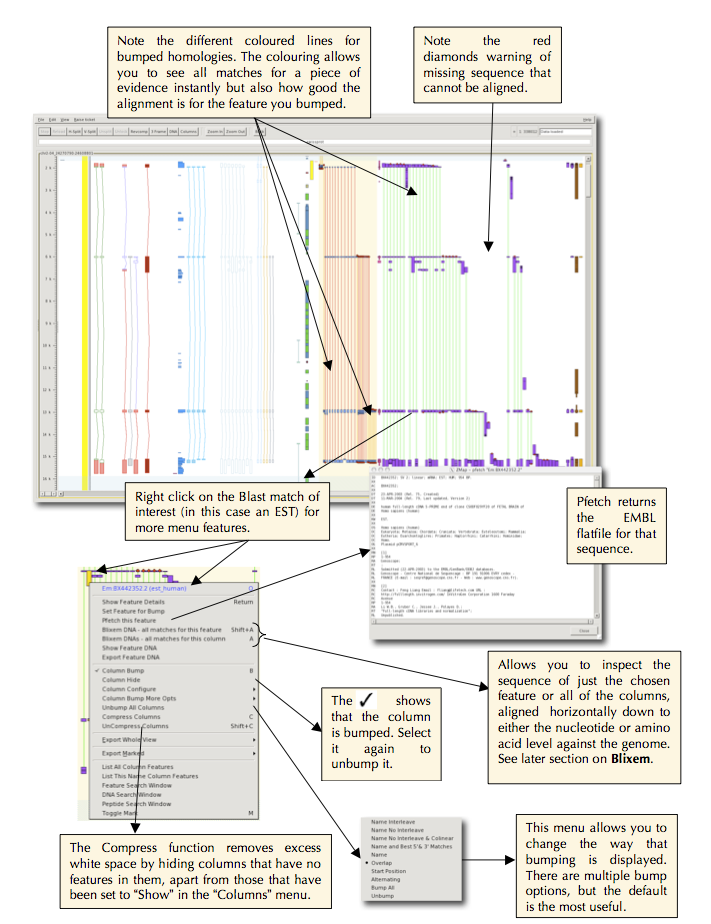
\includegraphics[width=15.231cm]{images/bumping.png}
\caption{Bumping features}
\label{img_bumping}
\end{figure}

Alignment quality of the HSPs is depicted by the width of every alignment displayed since the width is a measure of that HSP's score. Therefore, the wider it is the closer the score is to 100\%. The precise score is displayed in the ZMap details bar by clicking on the alignment. If HSPs are missing either the first or last Blast alignments in the set, they are marked with a red diamond at their start/end respectively. This indicates if they do not start at the first base/amino acid and/or do not end with the last base/amino acid of the alignment sequence. Figure \ref{img_bumping} shows what options you get when you right click over a homology. You also get further options such as retrieving the EMBL file for that homology using pfetch and starting \textbf{Blixem}; see section \ref{sec_blixem} (note, HSPs do not need to be bumped to use Blixem).


\subsection{Filter tracks} \label{sec_filter}
You can filter tracks by score using the Filter spinwheel box on the toolbar (see section \ref{sec_toolbar}). First, click in the column you want to filter so that it is highlighted. Then, either use the up/down buttons to change the desired cutoff, or simply type into the box directly to set the cutoff. The features in the column will be filtered so that only features that have a score equal to or greater than the cutoff will remain. Simply set the cutoff back to 0 to show all features again.

Columns that have filtered-out features can be highlighted in a different colour. Tick \lstinline{Highlight Filtered Columns} in the Preferences dialog to turn this highlighting on (see section \ref{sec_preferences_display}).


\subsection{Featureset styles and strand}
ZMap has rich feature display capabilities, which are highly configurable. Different features are displayed in distinct columns, and can be configured with many different styles as shown in figure \ref{img_features}. 

\begin{figure}
\centering
\color[rgb]{0.30980393,0.5058824,0.7411765}
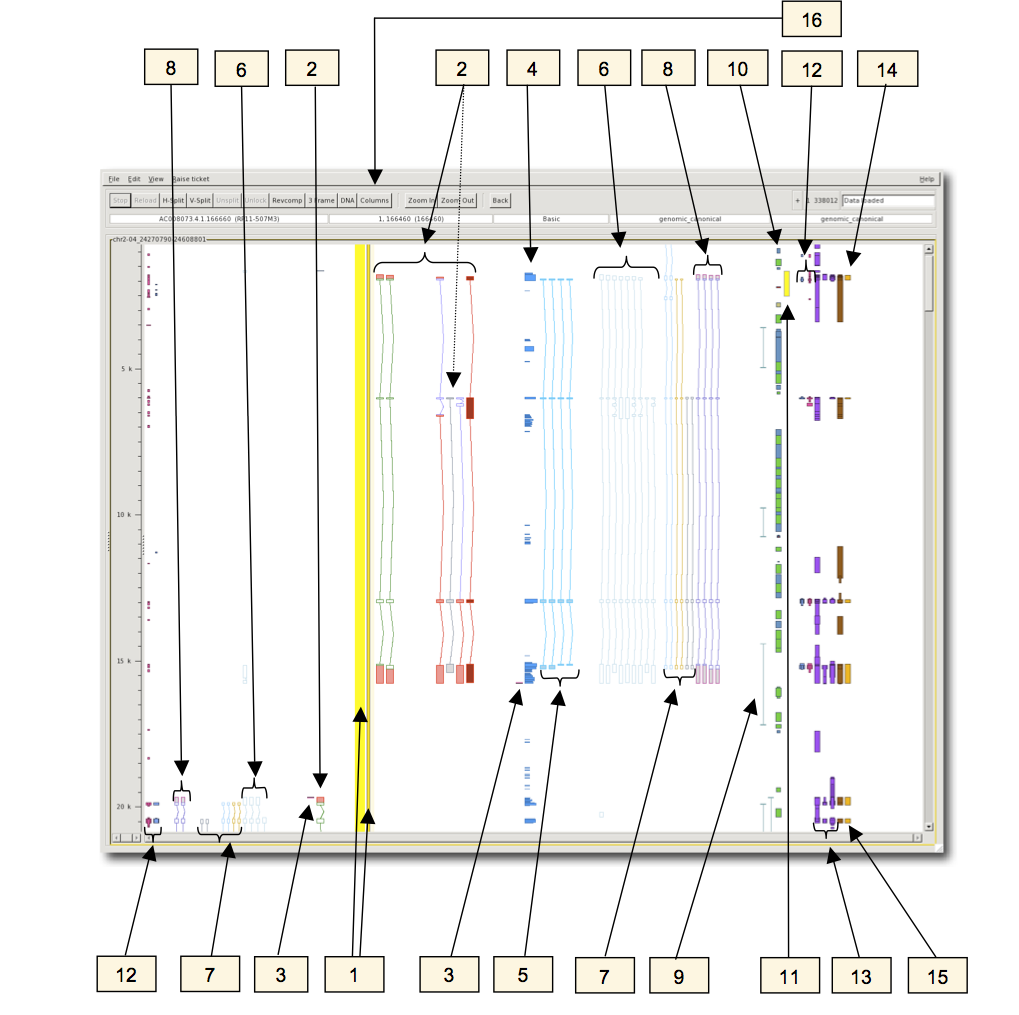
\includegraphics[width=15.231cm]{images/features.png}
\caption{Features}
\label{img_features}
\end{figure}

\begin{enumerate}
\item The thick yellow line represents the genomic sequence; everything to the left represents the reverse strand and everything to the right the forward strand. DNA matches (i.e. ESTs, mRNAs and RefSeq) and repeats have been configured so that they are all displayed on the current forward strand although they may align to either strand. Other features are configured to display only on their relevant strand. The thin bar to the right is the clone that the genomic sequence is made up from. When connected to the Otter peer, double-clicking on this gives access to the DE editing window.
\item Annotated transcripts; green is coding (CDS), red is non-coding (UTR and transcript variants) and purple shows the ``coding'' region of NMD variants. Grey transcripts (see dotted line) contain exons outside the sequence slice being viewed and should not be confused with Halfwise hits.
\item Curated features, such as PolyA features are seen as horizontal black lines.
\item Phastcons44 - conserved regions detected using multiple sequence alignments of 44 organisms.
\item Imported annotation from CCDS (human and mouse only).
\item Imported transcripts via DAS source. Here PASA\_ESTs are shown.
\item Predicted transcripts such as Genscan (pale blue), Augustus (gold) and Halfwise predictions of Pfam (grey).
\item Imported annotation from Ensembl.
\item gis\_pet\_ditags and chip\_pet\_ditags are indicators of transcript boundaries.
\item Repeats ( blue=Line , light green=Sine , gold=other ), tandem repeats are red.
\item CpG islands appear as yellow boxes.
\item Protein matches are strand specific - SwissProt are light blue and Trembl pink.
\item EST matches are displayed as purple blocks and are broken down into human ESTs, mouse ESTs, and other ESTs from other organisms. 5' reads are on the left and 3' on the right.
\item mRNA matches contains all species and are displayed as brown blocks,
\item RefSeq matches are the orange blocks.
\item View and configure columns (i.e. the available features and analysis) - see section \ref{sec_track_configuration}.
\end{enumerate}


\subsection{Track configuration} \label{sec_track_configuration}
The Column Configuration dialog (figure \ref{img_columns}) is used to control which tracks are displayed, to specify the order of columns, and to edit the style and other properties of the columns.  The dialog can be opened from the \lstinline{Columns} button on the toolbar, or via the right-click menu (\lstinline{Column Configuration->Configure this/all columns}).

\begin{figure}
\centering
\color[rgb]{0.30980393,0.5058824,0.7411765}
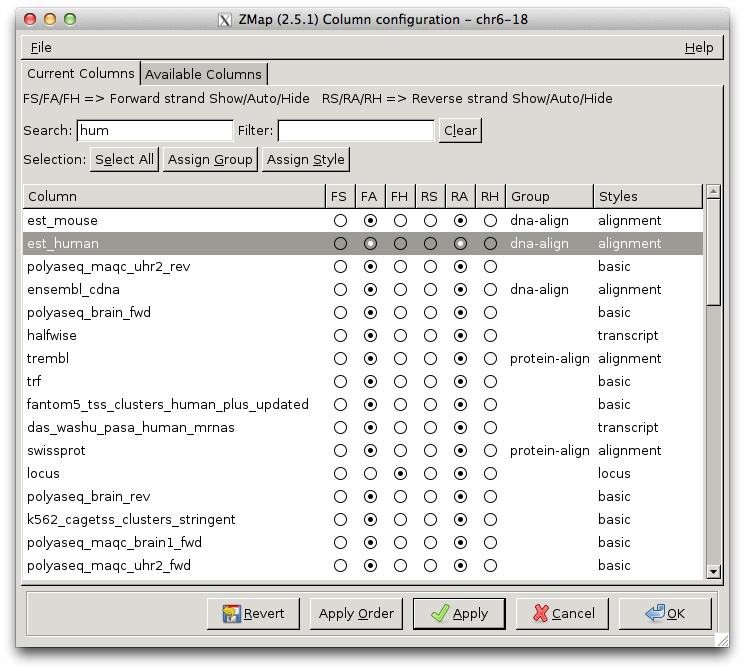
\includegraphics[resolution=150]{images/columns.png}
\caption{Column configuration dialog}
\label{img_columns}
\end{figure}

Each available track is listed and its visibility, group and style are shown.

\subsubsection{Selecting rows}
You can select one or more rows in the dialog to perform operations on them. To select multiple rows, you can hold down Ctrl (for one-by-one selection) or Shift (for range selection) while clicking with the mouse, or hold down Shift and press the up/down arrows.

\subsubsection{Search and filter rows}
You can quickly jump to a row containing specific text using the \lstinline{Search} box. As you type in the box, the row selection will jump to the first row containing that text. You can use the up/down arrows to jump to the next/previous matching row.

You can filter the displayed rows by specific text using the \lstinline{Filter} box. Type in the required text and press \lstinline{Enter} and the rows will be filtered. Click the \lstinline{Clear} button to clear the filter and go back to viewing all rows.

\subsubsection{Track visibility}
The visibility of each track (for both the forward and reverse strand) is controlled by a set of radio buttons with the options \lstinline{show}, \lstinline{auto} and \lstinline{hide}:
\begin{itemize}
\item \textbf{Show} - the column will always be visibile 
\item \textbf{Auto} - column visibility will be controlled automatically depending on the way the column is configured, e.g. the column may only be shown at certain levels of zoom
\item \textbf{Hide} - the column will always be hidden
\end{itemize}

To change the visibility, select the track(s) you want to change and then click the relevant radio button in any of the selected tracks. Note that all highlighted tracks will be changed.

Note that you can also hide a track directly from the ZMap canvas by right-clicking on the column and selecting \lstinline{Column Hide}.

\subsubsection{Assigning groups} \label{sec_groups}
You can assign a group to one or more tracks by selecting the tracks and clicking \lstinline{Assign Group}. You will be prompted to enter a name for the group. The new group name will be populated on the Columns dialog. Remember to click \lstinline{Apply} or \lstinline{OK} on the Columns dialog to apply the changes.

Groups are used by various operations in ZMap such as running Blixem (see section \ref{sec_blixem}). When you run Blixem on a column, you have the option of running it on ``associated columns''. This will run Blixem on all columns that are in the same group as the selected column.

\subsubsection{Assigning styles}
You can assign a style to one or more tracks by selecting the tracks and clicking \lstinline{Assign Style}. This will open the \lstinline{Choose Style} dialog where you can select the required style, or create a new one (see section \ref{sec_style_configuration}). After choosing a style, the new style name will be populated on the Columns dialog. Remember to click \lstinline{Apply} or \lstinline{OK} on the Columns dialog to apply the changes.

\subsubsection{Reordering tracks}
Tracks can be reordered by dragging and dropping rows in the Columns dialog. You can also sort the rows by name, group or style by clicking on the appropriate header. You must click the \lstinline{Apply Order} button to apply the new track order in ZMap. Note that the main \lstinline{Apply} and \lstinline{OK} buttons do NOT apply the column order in ZMap.

\subsubsection{Saving configuration}
Column configuration can be saved in one of two ways. To save the configuration to your general ZMap settings so that will apply in all future sessions, go use the menu option \lstinline{File->Save} on the \lstinline{Column configuration} dialog. Alternatively, to save the configuration to a separate config file, so that you can load it selectively in future, use the menu option \lstinline{File->Export->Configuration} from ZMap's main menu.


\subsection{Style configuration} \label{sec_style_configuration}
You can view and edit the styles of all featuresets in ZMap from the \lstinline{Styles} dialog. Open the dialog by going to the menu \lstinline{Edit->Styles}. You can also open the Styles dialog from the \lstinline{Column configuration} dialog by selecting \lstinline{Assign Style}.

All featuresets are assigned a default style on startup if they do not already have styles configured (see the styles.shtml help file for information about pre-configuring styles). Styles are usually organised into an heirarchy whereby child styles inherit the properties of their parent styles. The Styles dialog shows a tree of the styles heirarchy. The primary default styles, ``basic'', ``alignment'' and ``transcript'', are derived from ``root''. 

Existing styles can be edited by selecting the row in the Styles dialog and clicking the \lstinline{Edit} button. This will open the \lstinline{Edit Style} dialog (see section \ref{sec_edit_style}). You can add a new child style to the currently-selected row by clicking the \lstinline{Add} button, or delete the currently-selected style using the \lstinline{Delete} button.

\subsubsection{Editing styles} \label{sec_edit_style}
The \lstinline{Edit Style} dialog is opened from the \lstinline{Styles} dialog when you Edit or Add a style. It can also be opened by right-clicking on a feature and going to the menu options \lstinline{Column configuration->Edit Style}.

When editing an existing style, the new name will default to the same as the existing name. This can be changed if you want to rename the style. The list of featuresets that currently use the style are shown. This is so that you can be sure you want to edit the style for all of those featuresets.

If you do not want to change the style for of the featuresets you can create a new child style by clicking the \lstinline{Create child style} button. This style will be assigned to just the selected featureset (if editing the style of a particular feature), or will be assigned to no featuresets otherwise (in which case you can assign it to featuresets later e.g. via the \lstinline{Column configuration} dialog).

\subsubsection{Saving styles}
Styles can be saved to an .ini style configuration file. To do this, go to the menu \lstinline{File->Save->Styles}. To load the styles in a future ZMap session, set up a configuration file and use the \lstinline{stylesfile} key (see the configuration.shtml help file for details).


\clearpage
\section{Operations}

\subsection{Show feature details}
Right click on a gene object or \lstinline{o} key when highlighted to see information on otter IDs and Ensembl IDs. For BLAST hits, double click on the HSP to get the feature interface where you will find details on alignment and on what gene object the HSP has been assigned to as evidence, if any (see figure \ref{img_feature_details_dialog}).

\begin{figure}
\centering
\color[rgb]{0.30980393,0.5058824,0.7411765}
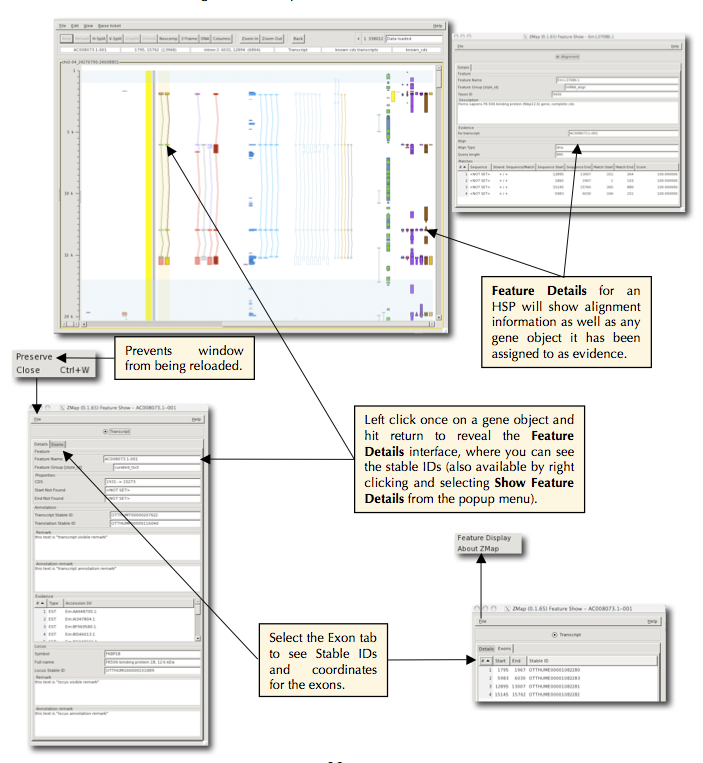
\includegraphics[width=15.231cm]{images/feature_details_dialog.png}
\caption{Feature details dialog}
\label{img_feature_details_dialog}
\end{figure}


\subsection{View/export sequence for gene objects} \label{sec_view_export_sequence}
There are various options for displaying or exporting the DNA or peptide sequence associated with a gene object. Note that you can edit a transcript's sequence before viewing/exporting it using ZMap's Annotation functionality (see section \ref{sec_edit_sequence}).

\begin{itemize}
\item You can \textbf{show the translation} of the gene model in the canvas alongside the model.
\item You can \textbf{view the DNA or peptide} sequence in pop up dialog boxes in ZMap.
\item You can \textbf{export the DNA or peptide} sequence to a FASTA file.
\end{itemize}

The \textbf{view} and \textbf{export} options are the same except that the output is either to the screen or to a file.

\subsubsection{Show translation} \label{sec_show_translation}
Right-click on a gene model and select \lstinline{Show Translation} to view the translation in the canvas. Alternatively, select a gene model and press the shortcut key \lstinline{t}. You can hide the column again with \lstinline{Shift-T}.

This will show a new column in ZMap showing the translation alongside the other features (see figure \ref{img_show_translation}). The introns are shown as dashes, and double-dashed lines are used in regions outside the transcript bounds.

Click on the gene model and the exons will be highlighted in the Show Translation column. The highlight colours are the same as in the 3-Frame column (see section \ref{sec_dna_3_frame}) with the exception that the darker green now indicates that the reading frame is the same as the feature's reading frame (as calculated from the start coordinate of the feature).

\begin{figure}
\centering
\color[rgb]{0.30980393,0.5058824,0.7411765}
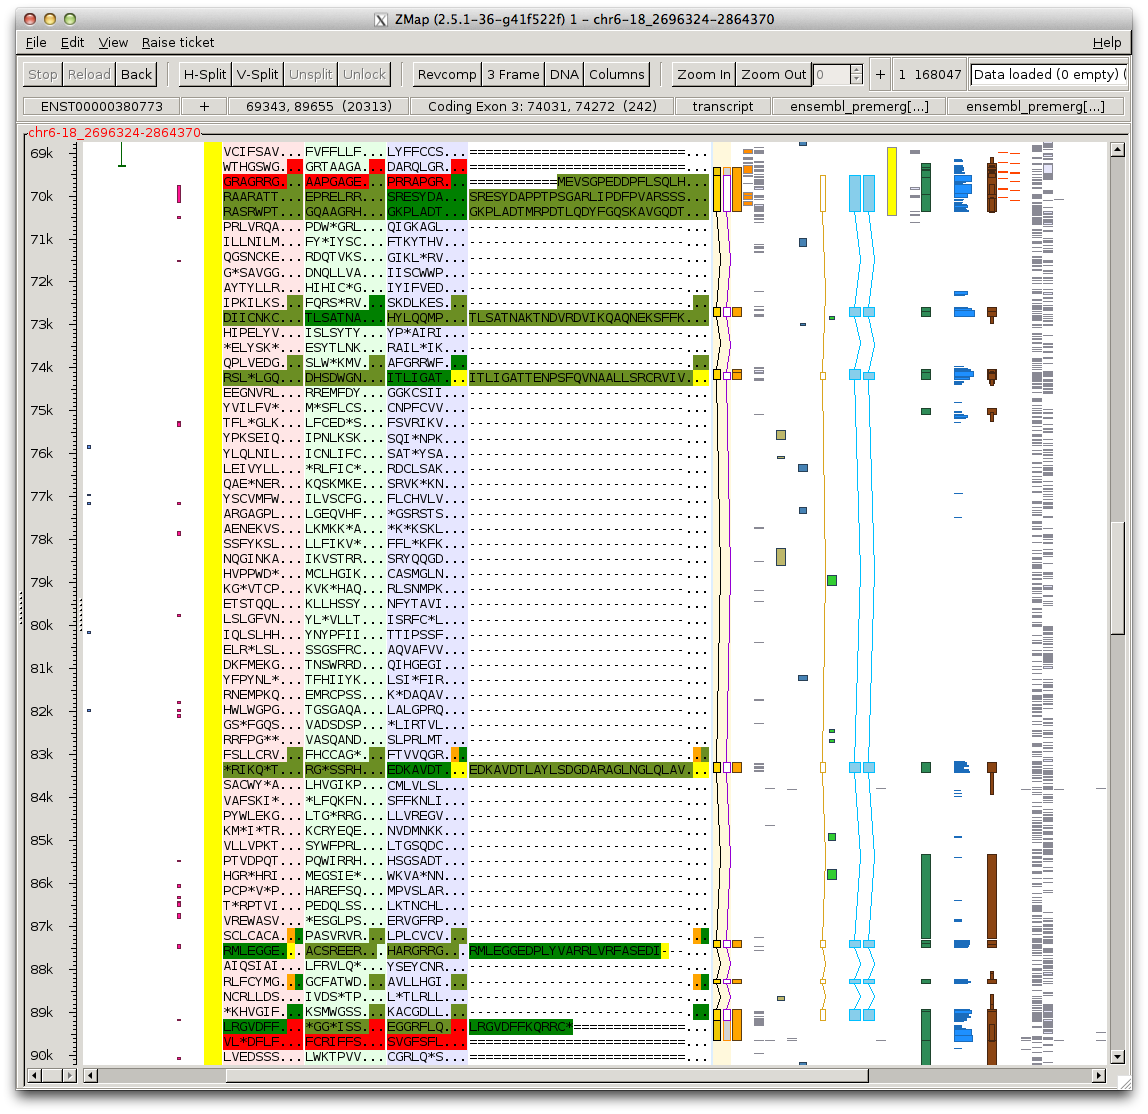
\includegraphics[width=15.231cm]{images/show_translation.png}
\caption{The Show Translation column (shown alongside the 3-frame tranlation on the left and the gene model on the right)}
\label{img_show_translation}
\end{figure}

\subsubsection{Feature DNA} \label{sec_feature_dna}
You can view or export the DNA sequence as one of the following:

\begin{itemize}
\item \textbf{CDS} - just the CDS
\item \textbf{transcript} - the whole spliced transcript, including UTR
\item \textbf{unspliced} - the whole unspliced transcript, including UTR and introns
\item \textbf{with flanking sequence} - the whole unspliced transcript, with flanking sequence at the start and end (whose length you will be prompted to specify)
\end{itemize}

The \textbf{view} options will open a dialog box in ZMap showing the sequence. As shown in figure \ref{img_view_dna}, the sequence is highlighted in the same colours as the DNA/3-Frame columns (see section \ref{sec_dna_3_frame}). The \textbf{export} options will allow you to dump the sequence directly to a FASTA file.

\begin{figure}
\centering
\color[rgb]{0.30980393,0.5058824,0.7411765}
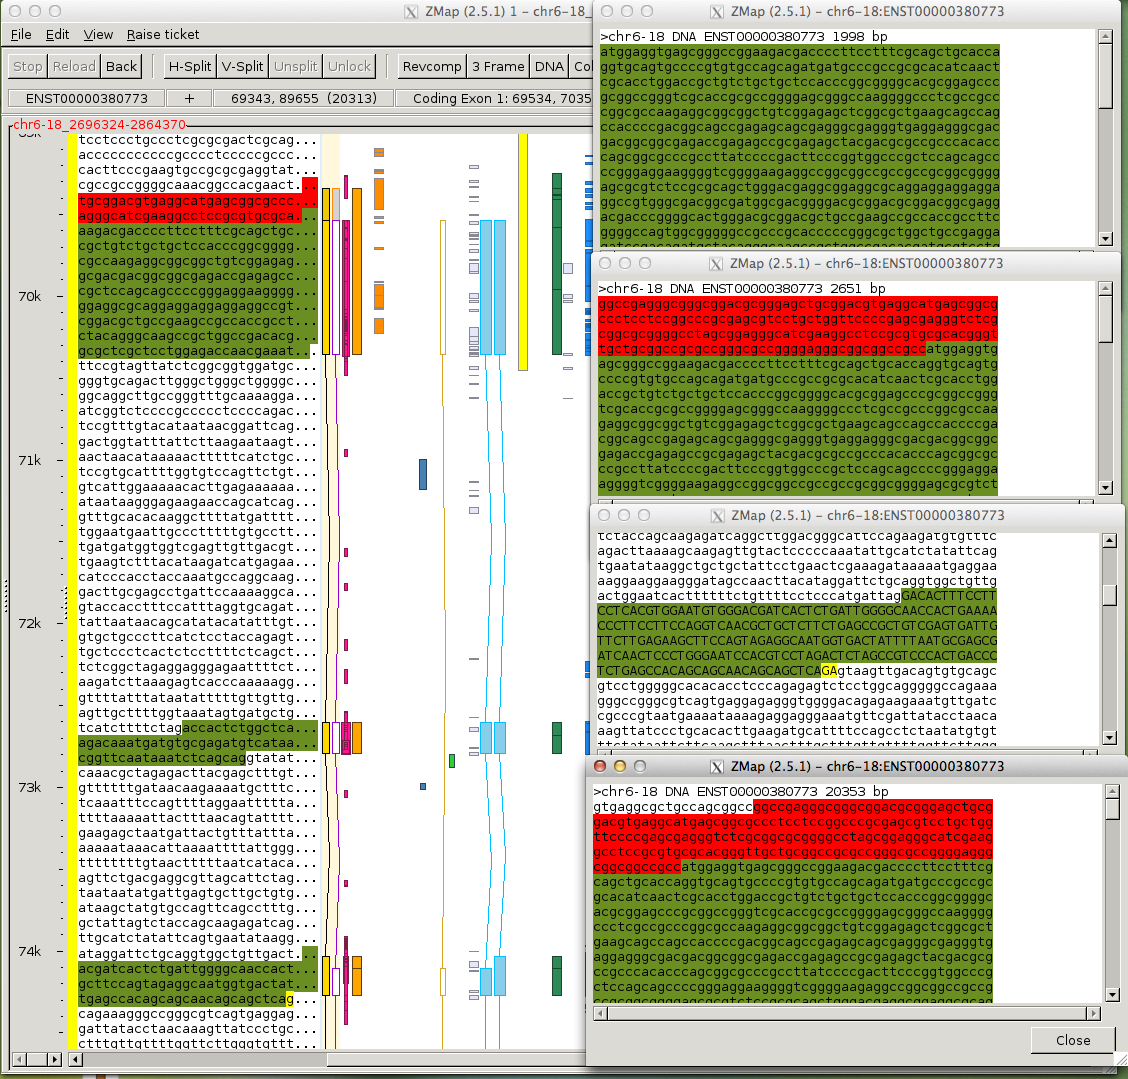
\includegraphics[width=15.231cm]{images/view_dna.png}
\caption{View DNA sequence: CDS; transcript; unspliced; with flanking sequence}
\label{img_view_dna}
\end{figure}

\subsubsection{Feature peptide} \label{sec_feature_peptide}
You can view or export the CDS as a peptide sequence. The \textbf{view} option will open a dialog box in ZMap showing the sequence (see figure \ref{img_view_peptide}). The \textbf{export} option will allow you to dump the sequence directly to a FASTA file.

\begin{figure}
\centering
\color[rgb]{0.30980393,0.5058824,0.7411765}
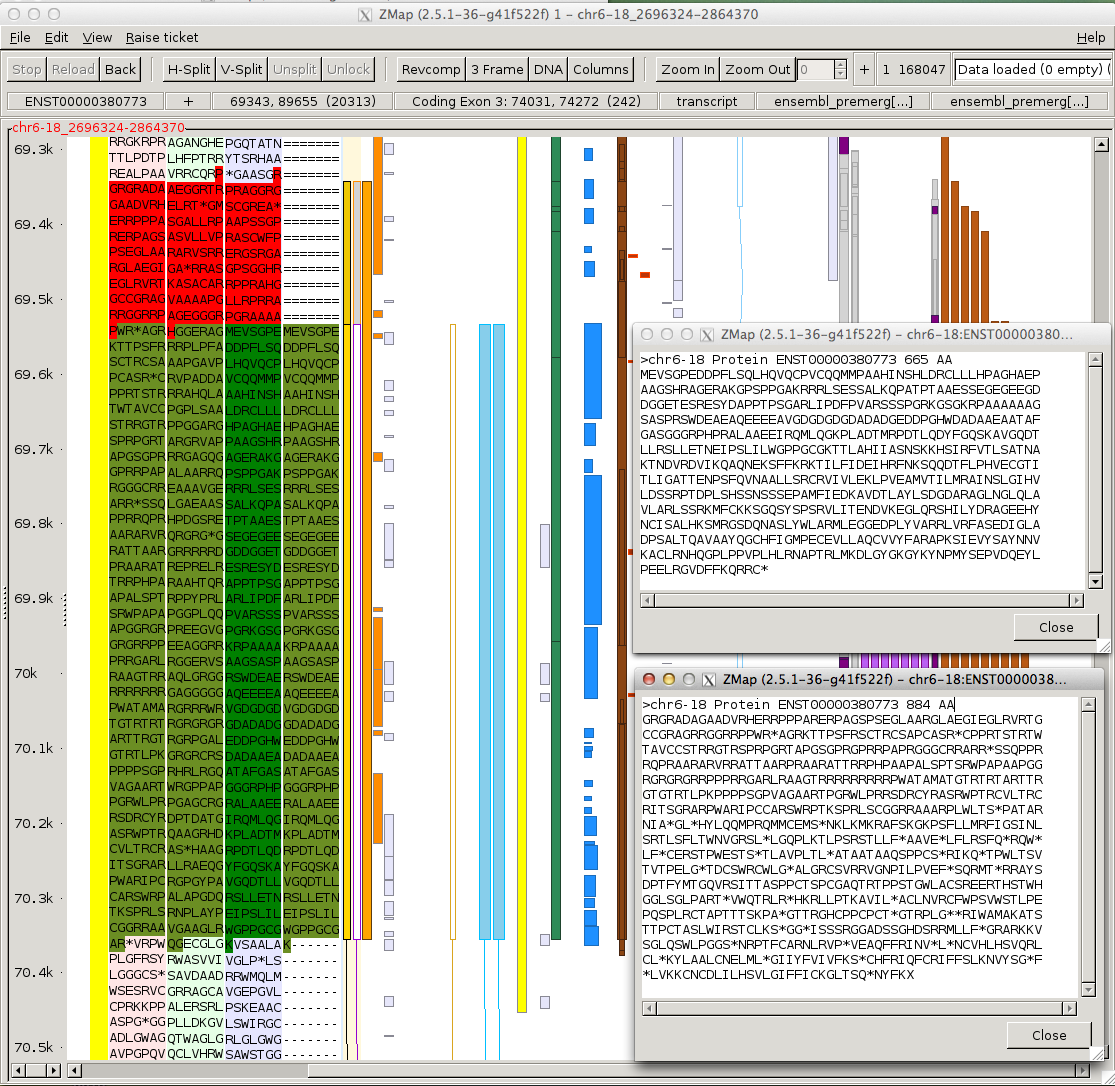
\includegraphics[width=15.231cm]{images/view_peptide.png}
\caption{View peptide sequence: CDS or whole transcript}
\label{img_view_peptide}
\end{figure}


\subsection{Exporting features to file}
You can export some or all of the features in ZMap to a GFF file. To export all features, go to the main menu and select \lstinline{File -> Export -> Features}. To export just a single feature, right click on that feature and go to \lstinline{View or Export... -> Export -> Clicked Feature}. To export all of the features in a column, right click on that column and go to \lstinline{View or Export... -> Export -> Column features}.


\subsection{Exporting reference DNA to file}
You can export the reference sequence DNA to a FASTA file. Go to the main menu and select \lstinline{File -> Export -> DNA}. 


\subsection{Searching for a sequence in ZMap}
DNA and peptide search windows are provided from within ZMap and can be accessed by right clicking on ZMap space and selecting the option at the bottom of the menu. Both search windows are shown in figure \ref{img_sequence_search}.

\begin{figure}
\centering
\color[rgb]{0.30980393,0.5058824,0.7411765}
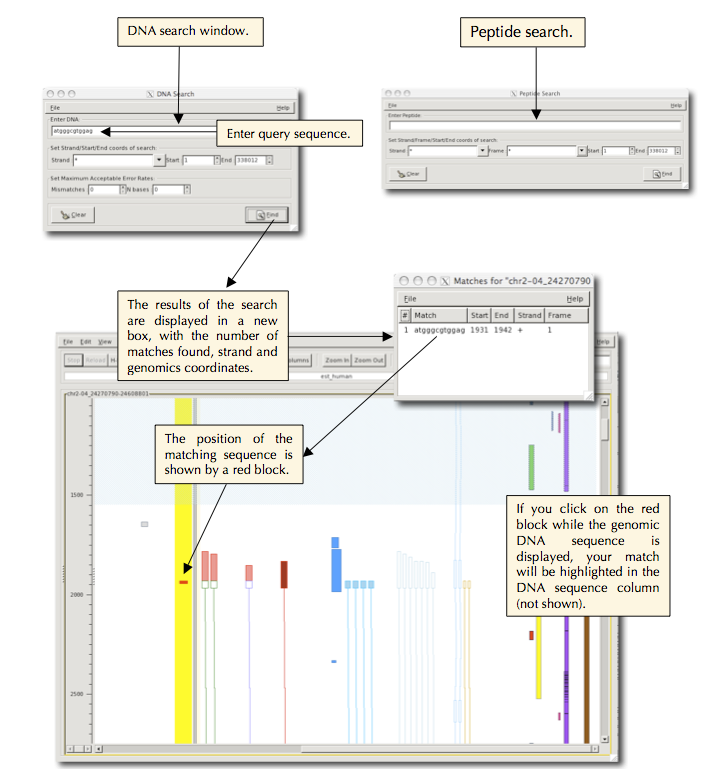
\includegraphics[width=15.231cm]{images/sequence_search.png}
\caption{Searching for a sequence}
\label{img_sequence_search}
\end{figure}


\subsection{Searching for a feature in ZMap}
This option allows you to list all the features contained in a column in one window. There are further options for you to search within these results to find a specific feature. The list of column features can be exported as a GFF file via the File menu. See figures \ref{img_feature_search} amd \ref{img_feature_search_results}.

\begin{figure}
\centering
\color[rgb]{0.30980393,0.5058824,0.7411765}
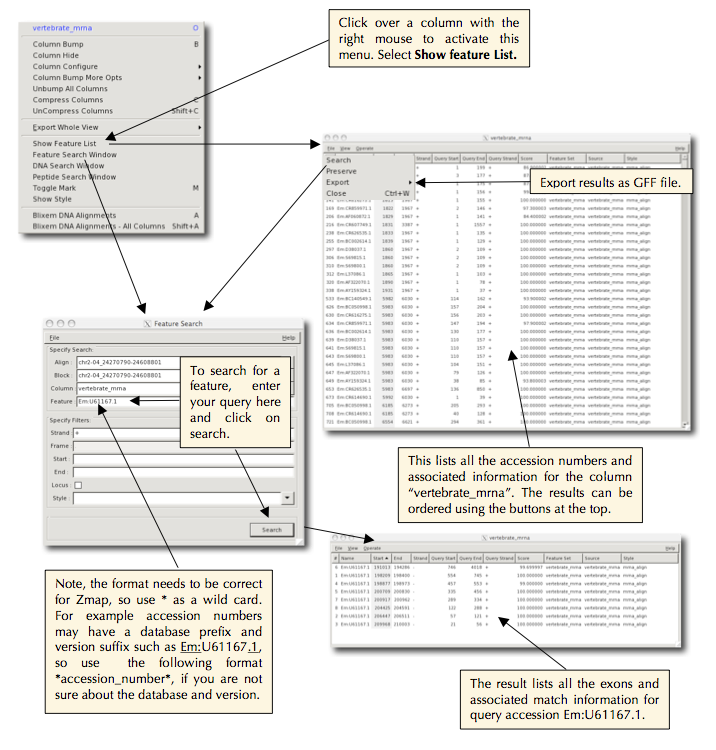
\includegraphics[width=15.231cm]{images/feature_search.png}
\caption{Searching for a feature}
\label{img_feature_search}
\end{figure}

\begin{figure}
\centering
\color[rgb]{0.30980393,0.5058824,0.7411765}
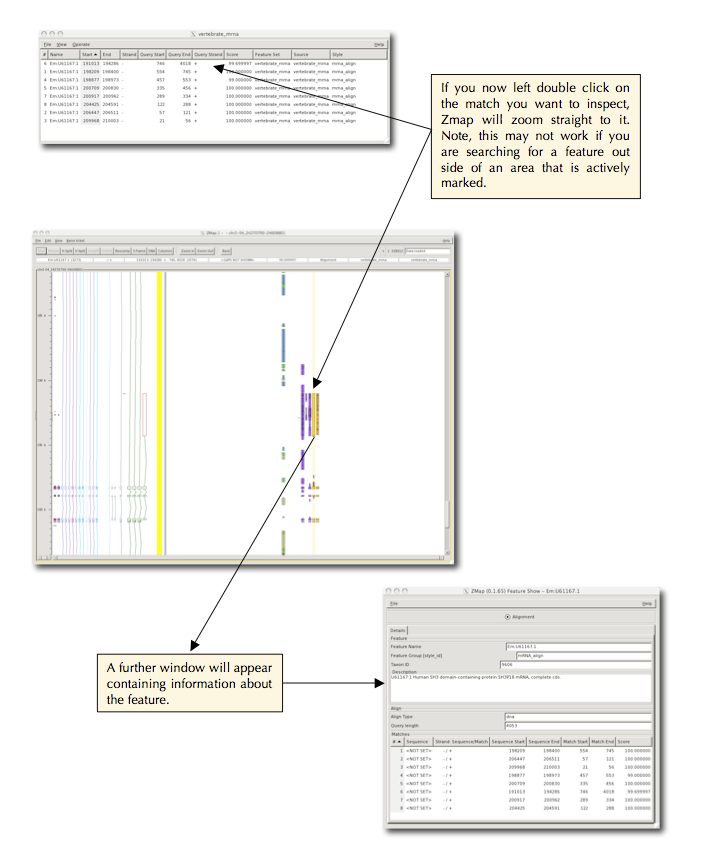
\includegraphics[width=15.231cm]{images/feature_search_results.png}
\caption{Feature search results}
\label{img_feature_search_results}
\end{figure}


\subsection{Use Blixem to view alignments in more detail} \label{sec_blixem}
ZMap does not store or display the sequence data for alignments. Instead, this can be viewed using Blixem. Blixem is an interactive browser of sequence alignments that have been stacked up in a ``master-slave'' multiple alignment; it is not a ``true'' multiple alignment but a ``one-to-many'' alignment.

Blixem can be easily started from ZMap on a single feature or an entire column. To start it, right-click on the feature/column of interest and select one of the following options (some of this may be under \lstinline{Blixem - more options}):
\begin{itemize}
\item \textbf{Blixem - all matches for this column} (\lstinline{A}) - All features in the current column
\item \textbf{Blixem - all matches for selected features} (\lstinline{Shift-A}) - The selected feature(s) only
\item \textbf{Blixem - all matches for associated columns} (\lstinline{Ctrl-A}) - All features in the same group as the current column (see section \ref{sec_groups} for details of how to set up groups)
\item \textbf{Blixem - all matches for selected features, expanded} (\lstinline{Shift-X}) - The selected feature(s), expanded into underlying data
\end{itemize}

Blixem will open up showing the specified alignments, along with any other featuresets it is configured to display e.g. transcripts (see the Blixem user manual for details about how to configure Blixem). It has a default scope of 200000 base pairs but this can be adjusted in the ZMap Preferences. From the preferences, you can also limit the features and/or scope to the marked region (see section \ref{sec_preferences_blixem}).


\clearpage
\section{Annotation} \label{sec_annotation}
ZMap can be used to create new features or edit existing features. ZMap can generate variant objects quickly - existing transcript objects can be used as a template for a new object while a ZMap HSP (or any other feature, nucleotide or peptide) can be used to provide the coordinates for the new variant. The annotation process is different depending on whether you are working within Otter or not.


\subsection{Standalone ZMap}
To create/edit features in ZMap, the workflow is roughly as follows:
\begin{itemize}
\item Enable Annotation
\item Copy a feature with \lstinline{Ctrl-K} to create a ``temporary feature''
\item Copy other features/coordinates to edit the temporary feature
\item Double-click the temporary feature to save it to a ``real'' featureset
\item Export the new feature to file
\end{itemize}

\subsubsection{Enable annotation}
To edit features in ZMap you must first enable annotation. Go to the menu option \lstinline{Edit -> Preferences} and tick \lstinline{Enable Annotation}. Alternatively, if you use the keyboard shortcut \lstinline{Ctrl-K} to copy your first feature to the Annotation column, then annotation will be enabled automatically.

\subsubsection{Create a temporary feature}
Features are edited by copying them to a \textbf{temporary feature} in the \textbf{Annotation} column (see figure \ref{img_editing_zmap}). The temporary feature can be based on any existing feature(s). The process is the same whether editing an existing gene model (in which case you will copy the gene model) or creating a new one (in which case you will copy the evidence features).

To create a new temporary feature, select the transcript (or other feature) you wish to create a variant from and press \lstinline{Ctrl-K} (or right-click and select \lstinline{Annotation -> Copy selected transcript(s)}\footnote{Note that you need to enable the Annotation column from the Preferences dialog for the Annotation menu to appear. Ctrl-K will automatically enable the Annotation column if it is not already enabled.}). Alternatively, you can create a transcript from an alignment (or any other feature) by clicking the alignment and pressing \lstinline{Ctrl-K} (or right-click and select \lstinline{Annotation -> Copy selected alignment(s)}).

\begin{figure}
\centering
\color[rgb]{0.30980393,0.5058824,0.7411765}
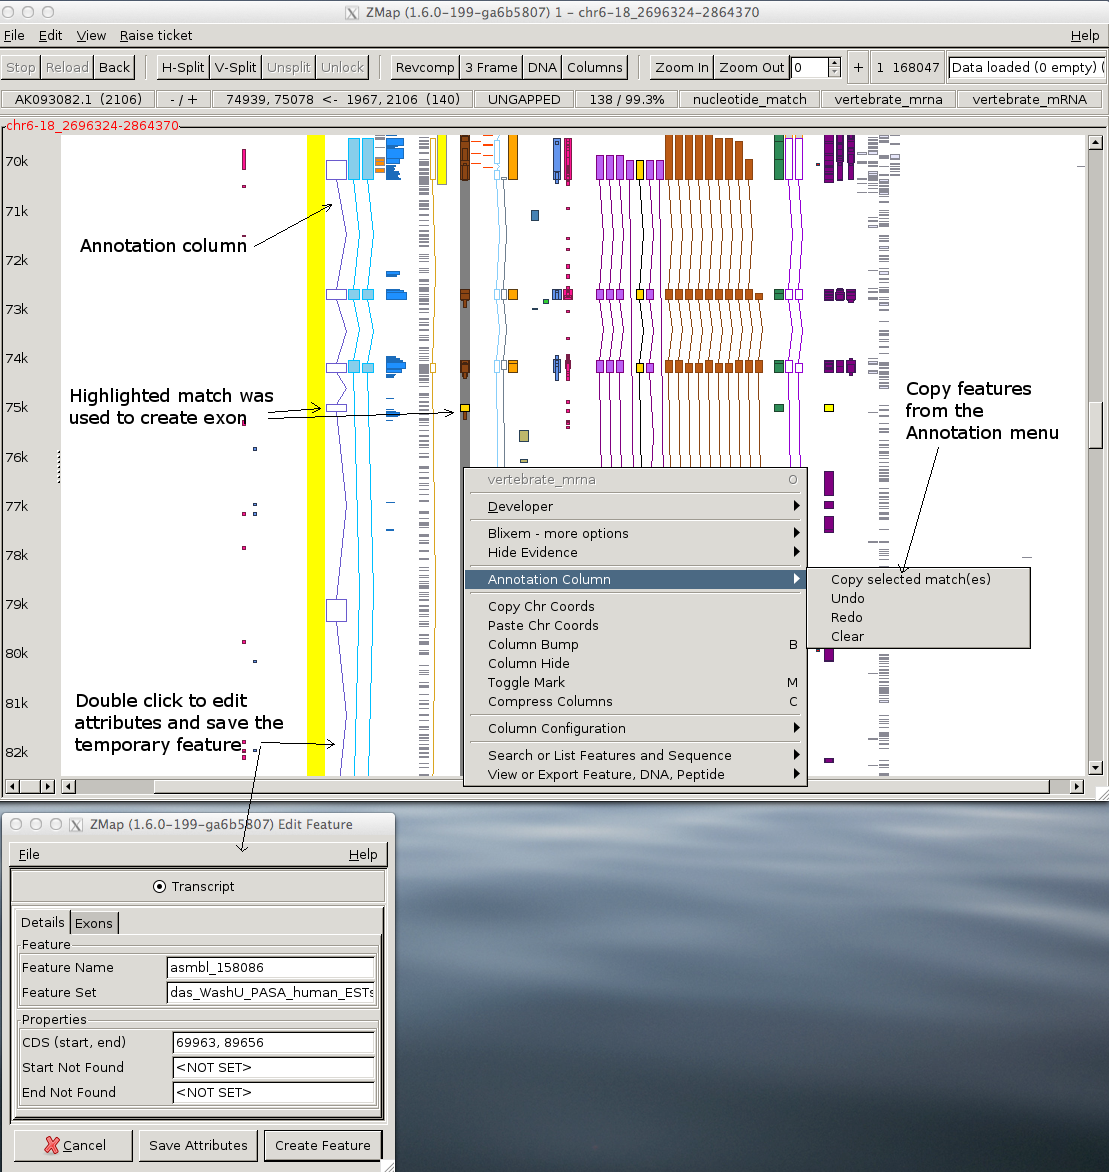
\includegraphics[width=15.231cm]{images/editing_zmap.png}
\caption{Feature editing in ZMap}
\label{img_editing_zmap}
\end{figure}

\subsubsection{Editing the coordinates}
Once you have created the temporary feature, it can be edited by copying additional features into the Annotation column in the same way. Objects of any time, including splice markers, nucleotide coords, peptide coords etc. can be used to adjust feature/exon coordinates. Select the other features you want to use and use \lstinline{Ctrl-K} or right-click and use the \lstinline{Annotation} menu to copy those in to adjust the coordinates of the original feature. You can copy the entire feature or just the selected sub-feature (e.g. the selected exon from a transcript or the selected hit from an alignment). You can use the keyboard shortcut \lstinline{Ctrl-K} to copy the entire feature. 

ZMap will do its best to make a sensible merge of the new coordinates, e.g. extending the feature extents if a coordinate lies outside the current range. If ZMap cannot automatically merge a coordinate it will ask for more information, e.g. if a coordinate lies within an intron, ZMap will ask whether it should form a 5' or 3' intron boundary.

You can delete exons and introns from the temporary feature by right-clicking on then and using the menu \lstinline{Annotation -> Delete subfeature}.

You can edit exon coordinates manually in the attributes dialog (see section \ref{sec_annotation_attributes}).

\subsubsection{Setting the CDS}
When you create the temporary feature, the CDS will be copied from the original feature, if it had one. The CDS can be edited in the attributes dialog (see section \ref{sec_annotation_attributes}). You can also set the CDS based on other features. To do this, right-click on the feature you want to base the CDS on and go to the menu \lstinline{Annotation -> Set CDS}. From here, you have the option to set just the \lstinline{Start} or \lstinline{End} of the CDS from this feature, or to set both (\lstinline{Range}). There is then a further option to choose whether you want to use the entire feature or just the clicked subfeature to set the CDS from.

\subsubsection{Editing the transcript's sequence} \label{sec_edit_sequence}
You can edit the transcript's sequence to see the effect of variation. This works by copying variation features into the Annotation column so you must have a variation column loaded. You will probably want to show the translation for the temporary feature first so you can see the effect of the changes. Click on the temporary feature and press \lstinline{t} to show the translation (or right-click on it and select \lstinline{Show Translation}). You may also want to show the three-frame translation (click the \lstinline{3 Frame} button on the toolbar to show it).

To apply a variation, right-click on the variation and go to the right-click menu \lstinline{Annotation -> Copy}. Select \lstinline{This feature} to copy just the clicked variation, or \lstinline{Selected feature(s)} to copy all selected features. You can use the keyboard shortcut \lstinline{Ctrl-K} to copy all selected features.

The object's translation will change to show the effect of the variation (see figure \ref{img_edit_sequence}). It may be useful to undo/redo the operation (see section \ref{sec_annotation_undo}) to see the translation before and after the change. You can view or export the edited sequence in the same way as any other gene model (see section \ref{sec_view_export_sequence}).

\begin{figure}
\centering
\color[rgb]{0.30980393,0.5058824,0.7411765}
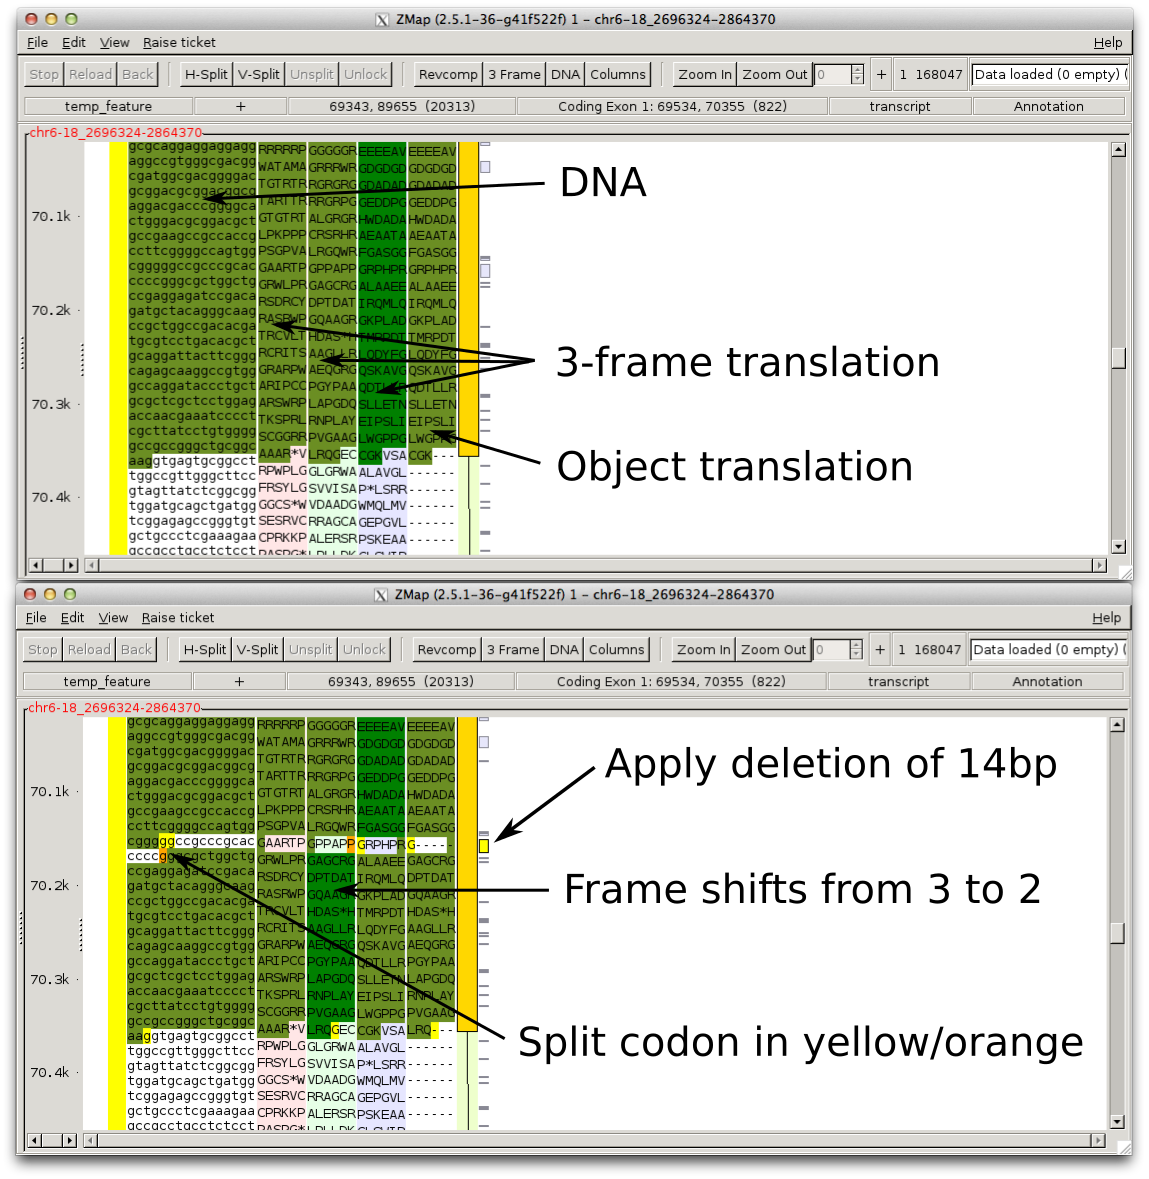
\includegraphics[width=15.231cm]{images/edit_sequence.png}
\caption{Editing a transcript's sequence. The variation highlighted in yellow (a deletion of 14bp) has been applied and has caused a frame-shift (as indicated by the shift of the dark green highlighting from frame 3 to frame 2). The yellow/orange bases indicate a split codon around the deletion.}
\label{img_edit_sequence}
\end{figure}

\subsubsection{Editing the attributes} \label{sec_annotation_attributes}
The coordinates and attributes of the temporary feature can be edited manually. Double-click the temporary feature to open a dialog showing its properties. Click on the \lstinline{Exons} tab, where you can then edit the exon coordinates. You can also edit other attributes such as the final feature name and featureset on this dialog as well. If you are not ready to save the feature to a featureset yet, you can save these attributes to the temporary feature by clicking \lstinline{Save Settings}. You can then continue editing the temporary feature, but the attributes will be remembered.

\subsubsection{Saving the temporary feature}
When you have finished editing your feature, you may wish to save it to a ``real'' featureset in ZMap so that you can clear the Annotation column and work on another transcript. You may then want to export either this single feature, or a group of features, to file. Alternatively, you may just wish to export the temporary feature directly to file. The process is different depending on what kind of save you want to do.

\textbf{Export the temporary feature}
If you just want to export the temporary feature to a GFF file, right-click on it and use the menu option \lstinline{Annotation -> Export temp feature}. You will then be able to choose a file to export the feature to. Only the temporary feature will be exported. Note that any attributes you set from the properties dialog.

\textbf{Save to a featureset}
When you have finished editing your feature, the temporary feature can be saved to a ``real'' featureset (i.e. to move it out of the Annotation column). Double-click the temporary feature to open a dialog showing its properties. To save it as a new feature, give it a new, unique name. To overwrite an existing feature, give it the same name and featureset as the feature you want to overwrite. ZMap will warn you before it overwrites an existing feature so you don't have to worry about overwriting one accidentally.

\textbf{Export to file}
Saving the temporary feature to a featureset moves it into the relevant column in ZMap. However, it is not saved to a file anywhere yet. To save it to file, you must export it to GFF. To export a single feature, right-click on it and use the menu option \lstinline{View or Export Feature... -> Export -> Clicked feature}. To save all features, go to the main menu and select \lstinline{File -> Export -> Features}. You will be prompted for a file name to save the feature(s) to.

\subsubsection{Other operations} \label{sec_annotation_undo}
\textbf{Undo/redo}
The right-click Annotation menu offers \lstinline{Undo} and \lstinline{Redo} options. These can also be accessed with the keyboard shortcuts \lstinline{Ctrl-Z} and \lstinline{Ctrl-Y}.

\textbf{Clear the Annotation column}
To clear the Annotation column ready to start again, right-click anywhere in ZMap and select \lstinline{Annotation -> Clear}. You may undo this operation if you select it by accident.

\textbf{Highlight evidence}
This option lets you highlight all of the feature(s) that were used to construct the temporary feature. Right-click on the temporary feature and select \lstinline{Highlight evidence}. The evidence features will be highlighted in yellow.


\subsection{Variant construction with Otter}
When running ZMap under Otter, variants are constructed in a different manner. See figures \ref{img_variant_construction} and \ref{img_variant_construction2}.

\begin{figure}
\centering
\color[rgb]{0.30980393,0.5058824,0.7411765}
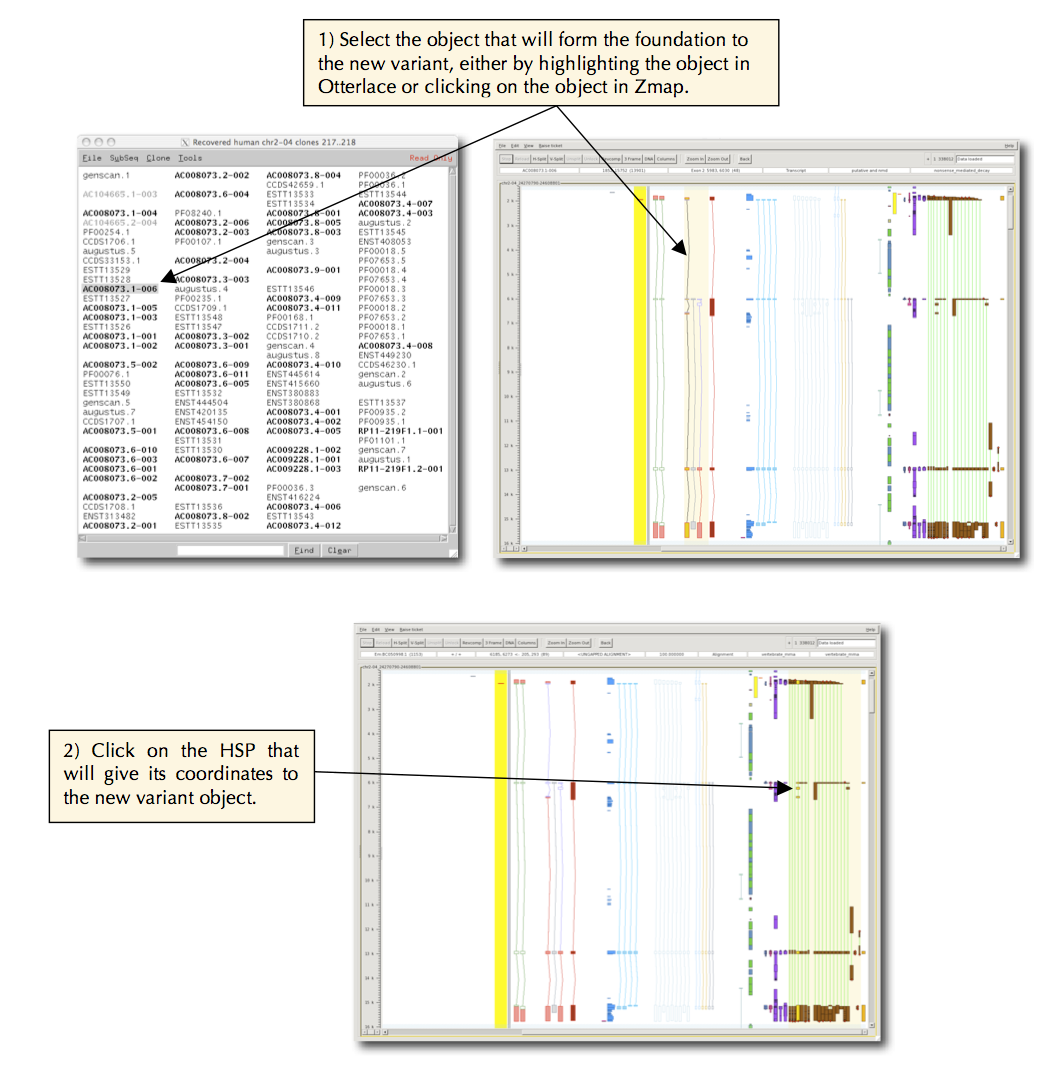
\includegraphics[width=15.231cm]{images/variant_construction.png}
\caption{Variant construction in Otter (1)}
\label{img_variant_construction}
\end{figure}

\begin{figure}
\centering
\color[rgb]{0.30980393,0.5058824,0.7411765}
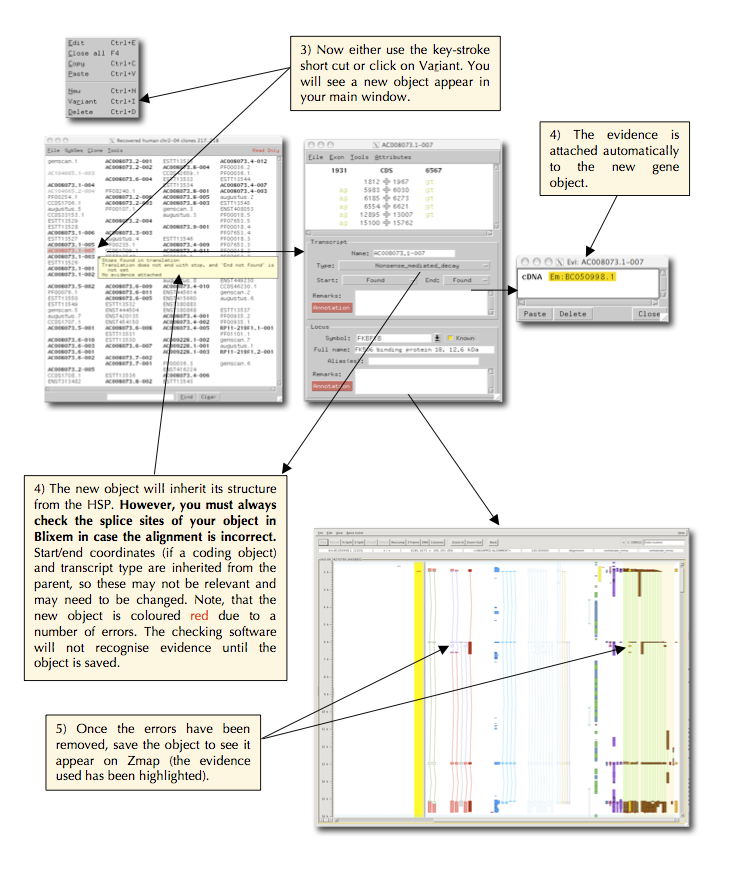
\includegraphics[width=15.231cm]{images/variant_construction2.png}
\caption{Variant construction in Otter (2)}
\label{img_variant_construction2}
\end{figure}


\clearpage
\section{Multiple views} \label{sec_multiple_views}
This function allows you to open two or more sequences alongside each other (such as a human region and the syntenic region in mouse, or two haplotypes), so that simultaneous investigation can be carried out. 


\subsection{Multiple views from GFF}
If you want have two different regions in GFF files, simply pass both GFF files to ZMap on the command line to view them side-by-side in ZMap:
\begin{lstlisting}
zmap file1.gff file2.gff
\end{lstlisting}


\subsection{Launching in a ZMap from Otter}
To open multiple sequences from Otter, you will need to open both sets of clones in the same Otter session. To open both ZMap windows in one window as shown below, you need to select ``Launch In A ZMap'' option in one clone set. These clones will open to the left of the already open Otter session. Figure \ref{img_launch_in_zmap} shows human gene SF3B14 and the syntenic region in mouse. The gene copy and paste function (referred to in the Otter section) is of much use here, saving time when building gene objects.

\begin{figure}
\centering
\color[rgb]{0.30980393,0.5058824,0.7411765}
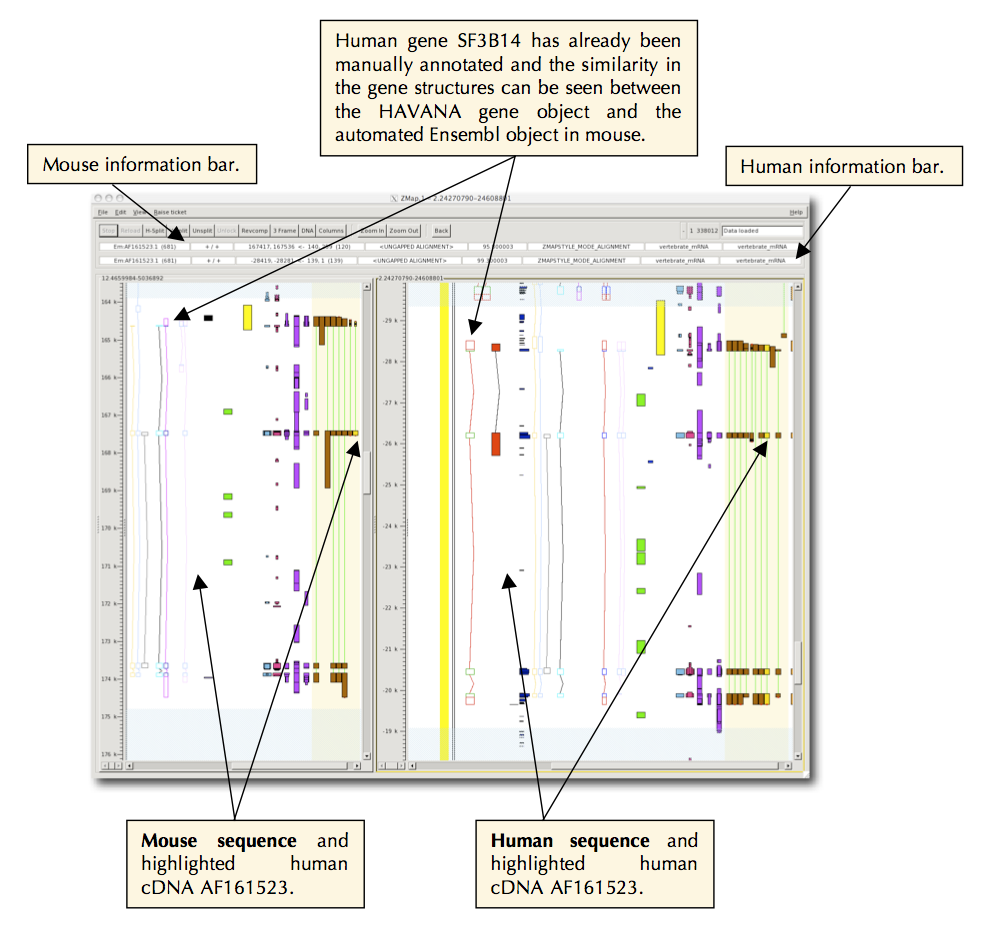
\includegraphics[width=15.231cm]{images/launch_in_zmap.png}
\caption{Launch in an existing ZMap}
\label{img_launch_in_zmap}
\end{figure}


\clearpage
\section{Preferences} \label{sec_preferences}
ZMap's preferences dialog can be shown by going to the main menu and selecting \lstinline{Edit -> Preferences}.

Preferences can be \textbf{saved} by going to the menu bar on the dialog and selecting \lstinline{File -> Save} (to save the current tab only) or \lstinline{File -> Save All} (to save all preferences). This will save your preferences for all future ZMap sessions until you overwrite them by changing them and saving again. Note that preferences are saved to the file \lstinline{~/.ZMap/zmap_prefs.ini}. This file can be deleted if you want to revert back to the default settings.


\subsection{Display preferences} \label{sec_preferences_display}
On the preferences dialog, select the \lstinline{Display} button to access the display preferences.

\subsubsection{Windows tab}
\begin{itemize}
\item \textbf{Shrinkable Window} - Allow the window to shrink more than the toolbar width (not recommended because some tools may be unavailable)
\item \textbf{Highlight Filtered Columns} - Highlight columns in a different colour when they contain features that have been filtered out (see section \ref{sec_filter})
\item \textbf{Enable Annotation} - Turn on feature editing functionality (see section \ref{sec_annotation})
\end{itemize}


\subsection{Blixem preferences} \label{sec_preferences_blixem}
On the preferences dialog, select the \lstinline{Blixem} button to access the Blixem preferences.

\subsubsection{General}
\begin{itemize}
\item \textbf{Scope} - Sets the maximum length of sequence to send to Blixem
\item \textbf{Restrict scope to Mark} - Restricts the scope to the current marked region
\item \textbf{Restrict features to Mark} - Still uses the default scope but only sends features that are within the marked region to Blixem
\item \textbf{Maximum Homols Shown} - Sets the maximum number of homologies that will be shown in Blixem
\end{itemize}

\subsubsection{Pfetch Socket Server}
The pfetch socket server is deprecated and will soon be removed.

\subsubsection{Advanced}
These settings are aimed at system administrators so should only be relevant to most users if you are setting up your own system or debugging problems. 

\begin{itemize}
\item \textbf{Config File} - Specify the location of the config file that Blixem should use
\item \textbf{Launch script} - Specify the location of the Blixem executable, if it is not in your path
\item \textbf{Keep temporary files} - ZMap creates temporary GFF files that it sends to Blixem. By default, Blixem will delete these, but if you tick this option it will not. Instead, they will be saved in a directory named \lstinline{/tmp/<user>_ZMAP_BLIXEM/}, where \lstinline{<user>} is your user ID.
\item \textbf{Sleep on Startup} - For debugging. This will pause Blixem for 10 seconds on startup so that a developer can attach a debugger.
\item \textbf{Kill Blixem on Exit} - If ticked, all Blixem's that were started from this ZMap will be closed when ZMap closes.
\end{itemize}


\clearpage
\section{Tips for a speedier ZMap}
\begin{enumerate}
\item Specifically: zoom and mark within ZMap early on after launching. Either select a gene object and press \lstinline{z} to zoom OR select a rectangle to zoom in by dragging the left mouse button around it. Reverse complement now if necessary, then press \lstinline{m} to mark the region.
\item The quickest way to zoom out of ZMap again is to right mouse click on the \lstinline{Zoom out} buttons at the top of zmap and choose one of the options (this is definitely much quicker that doing individual \lstinline{Zoom out}s with the left mouse button). Likewise for 'zooming in' again (or use keyboard equivalents).
\item Bump within a marked region only. Bumping without marking is slow and removes the lines connecting Blast matches.
\item When you have finished working within a marked region, unbump the evidence you have been working on (e.g. ESTs) and unmark that region before you go on to select the next region to mark and bump - or you could miss visualising the evidence in the new region.
\item If you want to get rid of some white space try the compress \lstinline{c} function or alternatively toggle off some of the columns. \textcolor{red}{Warning - this may hide features as well}. If a column (e.g ESTs) is bumped and you want to lose it temporarily, it is quicker to turn the column off (when you turn it on again it will still be bumped when it re-appears) than unbump then rebump again later.
\item Jumping to genes/objects: If you expand the left hand ``scroll navigator'' overview, you can jump directly to genes and objects by double-clicking on them.
\end{enumerate}


\clearpage
\section{Keyboard and mouse shortcuts}
In general ZMap will be faster for zooming, bumping etc if you make good use of the built in short cuts. These can often avoid the need for ZMap to redraw large amounts of data that you may not even be interested in. For example, click once (highlight) on a feature and a carriage return will bring up evidence. Another example is to press T for translation.


\subsection{All windows}

\begin{supertabular}{|m{6cm}|m{8.5cm}|}
\hline
Short Cut & Action \\
\hline
Cntl-W & close this window \\
Cntl-Q & quit ZMap \\
\hline
\end{supertabular}


\subsection{ZMap Window}

\begin{supertabular}{|m{6cm}|m{8.5cm}|}
\hline
Short Cut & Action\\
\hline
\multicolumn{2}{|l|}{Control keys} \\
\hline
+ (or =), - & zoom in/out by 10\%\\
Cntl + (or =), Cntl - & zoom in/out by 50\%\\
up-arrow, down-arrow & scroll up/down slowly bit\\
Cntl up-arrow, Cntl down-arrow & scroll up/down more quickly\\
left-arrow, right-arrow & scroll left/right slowly\\
Cntl left-arrow, Cntl right-arrow & scroll left/right more quickly\\
page-up, page-down (Mac users should use fn and up/down arrow) & up/down by half a ``page''\\
Cntl page-up, Cntl page-down & up/down by a whole ``page''\\
Home, End (Mac users should use fn and left/rights arrows) & Go to far left or right\\
Cntl Home, Cntl End (Mac users will have to configure their keyboards for this) & Go to top or bottom\\
Delete, Shift Delete & Hide/Show selected features.\\
Enter & Show feature details for highlighted feature.\\
Shift up-arrow, Shift down-arrow & Jump from feature to feature within a column.\\
Shift left-arrow, Shift right-arrow & Jump from column to column.\\
Cntl-K & Copy selected feature(s) to the Annotation column for editing. Also enables Annotation if not already enabled.\\
\hline
\end{supertabular}


\subsection{Alpha-numeric keys}
\begin{supertabular}{|m{1.5cm}|m{13cm}|}
\hline
Short Cut & Action\\\hline
a & Blixem all sequences in column\\
A & Blixem only highlighted sequence in column\\
b & Bump/unbump current column within limits of mark if set, otherwise bump the whole column.\\
B & Bump/unBump current column within limits of the visible feature range.\\
c & compress/uncompress columns: hides columns that have no features in them either within the marked region or if there is no marked region within the range displayed on screen. Note that columns set to ``Show'' will not be hidden.\\
C & Compress/unCompress columns: hides all columns that have no features in them within the range displayed on screen regardless of any column, zoom, mark etc. settings.\\
h & Toggles highlighting (good for screen shots).\\
m & mark/unmark a range which spans whichever features or subparts of features are currently selected for zooming/smart bumping\\
M & Mark/unMark the whole feature corresponding to the currently selected subpart (e.g. the whole transcript of an exon or all HSPs of the same sequence as the highlighted one) for zooming/smart bumping\\
o or O & show menu Options for highlighted feature or column, use cursor keys to move through menu, press ESC to cancel menu.\\
r & reverse complement current view, complement is done for all windows of current view.\\
t or T & translate highlighted item, T hides Translation.\\
w or W & zoom out to show whole sequence\\
z & zoom to the extent of any selected features (e.g. exon/introns, HSPs etc) or any rubberbanded area if there was one.\\
Z & Zoom to whole transcript or all HSPs of a selected feature.\\
\hline
\end{supertabular}


\subsection{ZMap Mouse Usage}
\begin{supertabular}{|m{4.8cm}|m{4.8cm}|m{4.8cm}|}
\hline
Left & Middle & Right\\
\hline
\textit{Single mouse button click} & & \\\hline
highlight a feature or column
Plus drag: draw a rectangle around an object for zoom &
horizontal ruler with sequence position displayed, on button release centre on mouse position.
Release mouse outside ZMap window to prevent re-centering.&
show feature or column menu - for options such as pfetch, show feature DNA, show peptide, export peptide\\
\hline
\textit{Double mouse button click} & & \\\hline
display details of selected feature. Double click on object to get edit window&
same as single click&
same as single click\\
\hline
\textit{Shift + mouse button click} & & \\\hline
highlight a subpart of a feature (e.g. a single exon or alignment match)
OR multiple highlight&
same as single click&
same as single click\\
\hline
\end{supertabular}


\end{document}
